
%%--------------------------------------------------
%% Serway: Physics for Scientists and Engineers
%%--------------------------------------------------


%% Chapter 05: The Laws of Motion
%%--------------------------------------------------


%% Table of Contents
%%--------------------------------------------------

%% 5.1 The Concept of Force
%% 5.1 Newton's First Law and Inertial Frames
%% 5.1 Mass
%% 5.1 Newton's Second Law
%% 5.1 The Gravitational Force and Weight
%% 5.1 Newton's Third Law
%% 5.1 Some Applications of Newton's Laws
%% 5.1 Forces of Friction


%% Serway Multiple Choice Questions
%%--------------------------------------------------
\element{serway-mc}{
\begin{question}{serway-ch05-q01}
    In the figure below,
    \begin{center}
    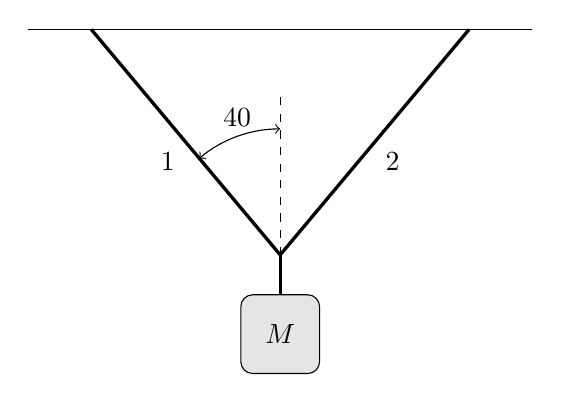
\begin{tikzpicture}[scale=0.8]
        %% Nodes
        \coordinate (A) at (-3,0);
        \coordinate (B) at (+3,0);
        \coordinate (C) at (0,-3.58);
        %% Rope
        \draw (-4,0) -- (4,0);
        \draw[very thick] (A) -- (C) node[anchor=north east,pos=0.5] {1};
        \draw[very thick] (B) -- (C) node[anchor=north west,pos=0.5] {2};
        \draw[dashed] (C) -- ++ (90:2.5);
        \draw[<->] (C) ++ (90:2) arc (90:130:2cm) node[pos=0.5,anchor=south] {\ang{40}};
        %% Mass
        \node[draw,fill=white!90!black,rectangle,rounded corners=1ex,minimum size=1cm,anchor=north,yshift=-0.5cm] (M) at (C) {$M$};
        \draw[very thick] (M.north) -- (C);
    \end{tikzpicture}
    \end{center}
        if the tension in string 1 is \SI{34}{\newton} and the tension in string 2 is \SI{24}{\newton},
        what is the mass of the object shown?
    \begin{multicols}{3}
    \begin{choices}
        \wrongchoice{\SI{7.3}{\kilo\gram}}
        \wrongchoice{\SI{5.5}{\kilo\gram}}
        \wrongchoice{\SI{1.8}{\kilo\gram}}
      \correctchoice{\SI{3.7}{\kilo\gram}}
        \wrongchoice{\SI{4.5}{\kilo\gram}}
    \end{choices}
    \end{multicols}
\end{question}
}

\element{serway-mc}{
\begin{question}{serway-ch05-q02}
    If $M = \SI{2.0}{\kilo\gram}$,
        what is the tension in string 1?
    \begin{center}
    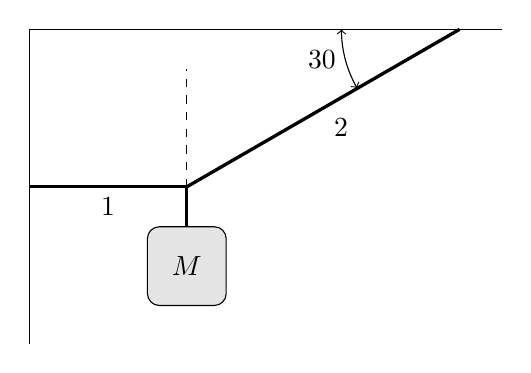
\begin{tikzpicture}
        %% Nodes
        \coordinate (A) at (0,0);
        \coordinate (B) at (+5.464,0);
        \coordinate (C) at (2,-2);
        \coordinate (D) at (0,-2);
        %% Lines
        \draw (0,0) -- (6,0);
        \draw (0,0) -- (0,-4);
        \draw[very thick] (B) --  (C) node[pos=0.5,anchor=north west] {2};
        \draw[very thick] (C) --  (D) node[pos=0.5,anchor=north] {1};
        \draw[dashed] (C) -- ++(90:1.5);
        \draw[<->] (B) ++ (210:1.5) arc (210:180:1.5) node[pos=0.5,anchor=east] {\ang{30}};
        %% Mass
        \node[draw,fill=white!90!black,rectangle,rounded corners=1ex,minimum size=1cm,anchor=north,yshift=-0.5cm] (M) at (C) {$M$};
        \draw[very thick] (M.north) -- (C);
    \end{tikzpicture}
    \end{center}
    \begin{multicols}{3}
    \begin{choices}
        \wrongchoice{\SI{1.2}{\newton}}
        \wrongchoice{\SI{11}{\newton}}
      \correctchoice{\SI{34}{\newton}}
        \wrongchoice{\SI{3.5}{\newton}}
        \wrongchoice{\SI{40}{\newton}}
    \end{choices}
    \end{multicols}
\end{question}
}

\element{serway-mc}{
\begin{question}{serway-ch05-q03}
    If $M = \SI{6.0}{\kilo\gram}$,
        what is the tension in string 1?
    \begin{center}
    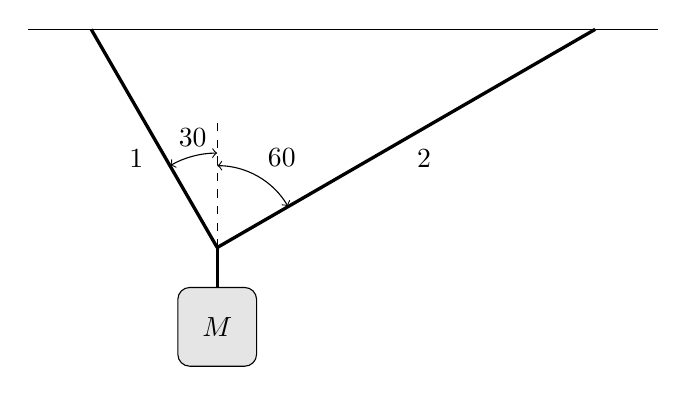
\begin{tikzpicture}[scale=0.8]
        %% Nodes
        \coordinate (A) at (-2,0);
        \coordinate (B) at (+6,0);
        \coordinate (C) at (0,-3.464);
        %% Lines
        \draw (-3,0) -- (7,0);
        \draw[very thick] (B) --  (C) node[pos=0.5,anchor=north west] {2};
        \draw[very thick] (C) --  (A) node[pos=0.5,anchor=north east] {1};
        \draw[dashed] (C) -- ++(90:2.0);
        \draw[<->] (C) ++ (90:1.5) arc (90:120:1.5) node[pos=0.5,anchor=south] {\ang{30}};
        \draw[<->] (C) ++ (90:1.3) arc (90:30:1.3) node[pos=0.5,anchor=south west] {\ang{60}};
        %% Mass
        \node[draw,fill=white!90!black,rectangle,rounded corners=1ex,minimum size=1cm,anchor=north,yshift=-0.5cm] (M) at (C) {$M$};
        \draw[very thick] (M.north) -- (C);
    \end{tikzpicture}
    \end{center}
    \begin{multicols}{3}
    \begin{choices}
        \wrongchoice{\SI{39}{\newton}}
        \wrongchoice{\SI{34}{\newton}}
        \wrongchoice{\SI{29}{\newton}}
        \wrongchoice{\SI{44}{\newton}}
      \correctchoice{\SI{51}{\newton}}
    \end{choices}
    \end{multicols}
\end{question}
}

\element{serway-mc}{
\begin{question}{serway-ch05-q04}
    If $M = \SI{1.1}{\kilo\gram}$,
        what is the tension in string 1?
    \begin{center}
    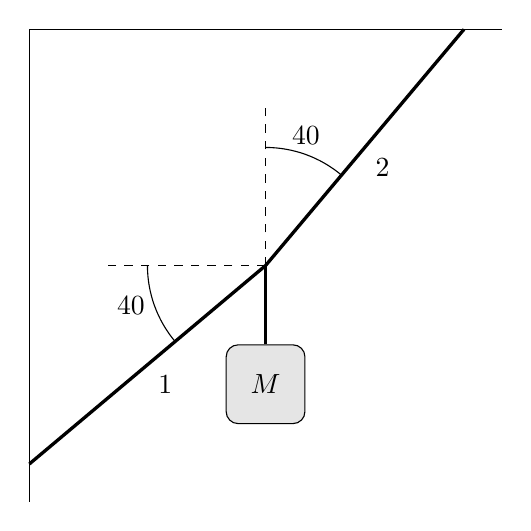
\begin{tikzpicture}
        %% Nodes
        \coordinate (A) at (0,0);
        \coordinate (B) at (+5.52,0);
        \coordinate (C) at (3,-3);
        \coordinate (D) at (0,-5.52);
        %% Lines
        \draw (0,0) -- (6,0);
        \draw (0,0) -- (0,-6);
        \draw[very thick] (B) --  (C) node[pos=0.5,anchor=north west] {2};
        \draw[very thick] (C) --  (D) node[pos=0.5,anchor=north west] {1};
        \draw[dashed] (C) -- ++(90:2.0);
        \draw (C) ++ (90:1.5) arc (90:50:1.5) node[pos=0.5,anchor=south] {\ang{40}};
        \draw (C) ++ (180:1.5) arc (180:220:1.5) node[pos=0.5,anchor=east] {\ang{40}};
        \draw[dashed] (C) -- ++(180:2.0);
        %% Mass
        \node[draw,fill=white!90!black,rectangle,rounded corners=1ex,minimum size=1cm,anchor=north,yshift=-1cm] (M) at (C) {$M$};
        \draw[very thick] (M.north) -- (C);
    \end{tikzpicture}
    \end{center}
    \begin{multicols}{3}
    \begin{choices}
        \wrongchoice{\SI{54}{\newton}}
        \wrongchoice{\SI{47}{\newton}}
      \correctchoice{\SI{40}{\newton}}
        \wrongchoice{\SI{62}{\newton}}
        \wrongchoice{\SI{57}{\newton}}
    \end{choices}
    \end{multicols}
\end{question}
}

\element{serway-mc}{
\begin{question}{serway-ch05-q05}
    An object of unknown weight is suspended as shown. 
    The tension in rope 1 is \SI{25}{\pound},
        and the tension in rope 2 is \SI{31}{\pound}. 
    What is the weight of the suspended object?
    \begin{center}
    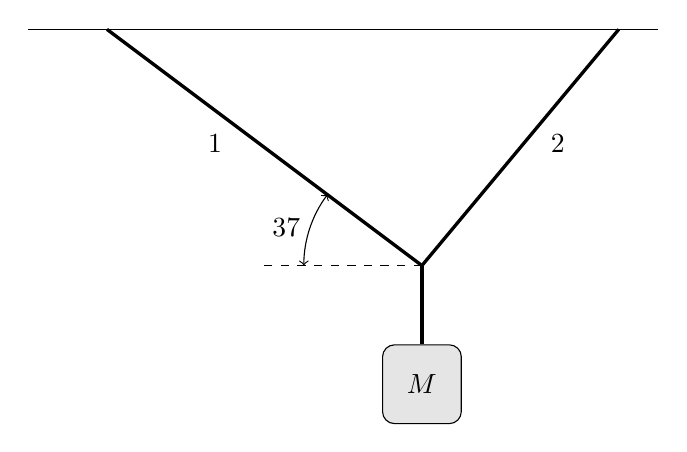
\begin{tikzpicture}
        %% Nodes
        \coordinate (A) at (-4.0,0);
        \coordinate (B) at (2.5,0);
        \coordinate (C) at (0,-3);
        %% Lines
        \draw (-5,0) -- (3,0);
        \draw[very thick] (A) -- (C) node[pos=0.4,anchor=north east] {1};
        \draw[very thick] (B) -- (C) node[pos=0.4,anchor=north west] {2};
        \draw[dashed] (C) -- ++(180:2);
        \draw[<->] (C) ++ (180:1.5) arc (180:143:1.5)
            node[pos=0.5,anchor=east] {\ang{37}};
        %% Mass
        \node[draw,fill=white!90!black,rectangle,rounded corners=1ex,minimum size=1cm,anchor=north,yshift=-1cm] (M) at (C) {$M$};
        \draw[very thick] (M.north) -- (C);
    \end{tikzpicture}
    \end{center}
    \begin{multicols}{3}
    \begin{choices}
        \wrongchoice{\SI{36}{\pound}}
        \wrongchoice{\SI{33}{\pound}}
        \wrongchoice{\SI{41}{\pound}}
      \correctchoice{\SI{39}{\pound}}
        \wrongchoice{\SI{56}{\pound}}
    \end{choices}
    \end{multicols}
\end{question}
}

\element{serway-mc}{
\begin{question}{serway-ch05-q06}
    If $\alpha=\ang{40}$, $\beta=\ang{60}$, and $M=\SI{4.0}{\kilo\gram}$,
        determine the tension in string 1.
    \begin{center}
    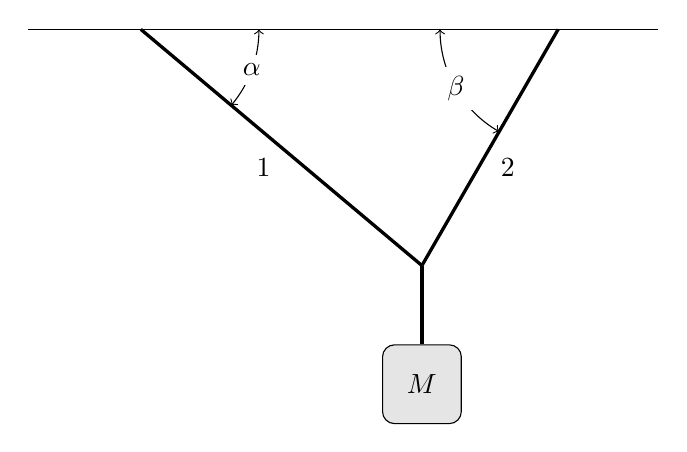
\begin{tikzpicture}
        %% Nodes
        \coordinate (A) at (-3.57,0);
        \coordinate (B) at (1.73,0);
        \coordinate (C) at (0,-3);
        %% Lines
        \draw (-5,0) -- (3,0);
        \draw[very thick] (A) -- (C) node[pos=0.5,anchor=north east] {1};
        \draw[very thick] (B) -- (C) node[pos=0.5,anchor=north west] {2};
        \draw[<->] (A) ++ (0:1.5) arc (0:-40:1.5) node[fill=white,pos=0.5,anchor=center] {$\alpha$};
        \draw[<->] (B) ++ (180:1.5) arc (180:240:1.5) node[fill=white,pos=0.5,anchor=center] {$\beta$};
        %% Mass
        \node[draw,fill=white!90!black,rectangle,rounded corners=1ex,minimum size=1cm,anchor=north,yshift=-1cm] (M) at (C) {$M$};
        \draw[very thick] (M.north) -- (C);
    \end{tikzpicture}
    \end{center}
    \begin{multicols}{3}
    \begin{choices}
        \wrongchoice{\SI{15}{\newton}}
        \wrongchoice{\SI{22}{\newton}}
        \wrongchoice{\SI{17}{\newton}}
      \correctchoice{\SI{20}{\newton}}
        \wrongchoice{\SI{36}{\newton}}
    \end{choices}
    \end{multicols}
\end{question}
}

\element{serway-mc}{
\begin{question}{serway-ch05-q07}
    If $\alpha=\ang{40}$ and the tension in string 2 is \SI{30}{\newton},
        determine $M$.
    \begin{center}
    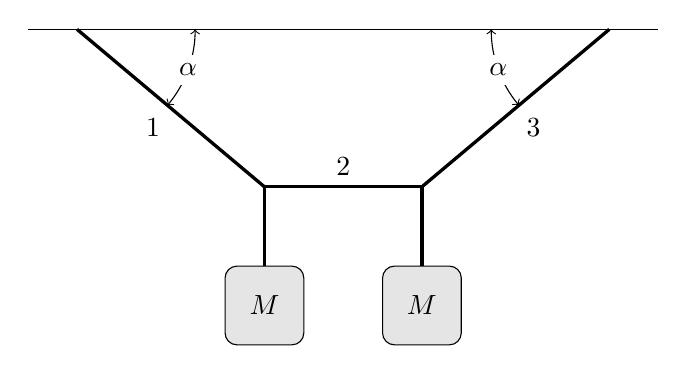
\begin{tikzpicture}
        %% Nodes
        \coordinate (A) at (-3.38,0);
        \coordinate (B) at (+3.38,0);
        \coordinate (C) at (-1,-2);
        \coordinate (D) at (+1,-2);
        %% Lines
        \draw (-4,0) -- (4,0);
        \draw[very thick] (A) -- (C) node[pos=0.5,anchor=north east] {1};
        \draw[very thick] (C) -- (D) node[pos=0.5,anchor=south] {2};
        \draw[very thick] (B) -- (D) node[pos=0.5,anchor=north west] {3};
        \draw[<->] (A) ++ (0:1.5) arc (0:-40:1.5) node[fill=white,pos=0.5,anchor=center] {$\alpha$};
        \draw[<->] (B) ++ (180:1.5) arc (180:220:1.5) node[fill=white,pos=0.5,anchor=center] {$\alpha$};
        %% Mass
        \node[draw,fill=white!90!black,rectangle,rounded corners=1ex,minimum size=1cm,anchor=north,yshift=-1cm] (M) at (C) {$M$};
        \node[draw,fill=white!90!black,rectangle,rounded corners=1ex,minimum size=1cm,anchor=north,yshift=-1cm] (N) at (D) {$M$};
        \draw[very thick] (M.north) -- (C);
        \draw[very thick] (N.north) -- (D);
    \end{tikzpicture}
    \end{center}
    \begin{multicols}{3}
    \begin{choices}
        \wrongchoice{\SI{3.4}{\kilo\gram}}
        \wrongchoice{\SI{3.6}{\kilo\gram}}
      \correctchoice{\SI{2.6}{\kilo\gram}}
        \wrongchoice{\SI{4.9}{\kilo\gram}}
        \wrongchoice{\SI{7.5}{\kilo\gram}}
    \end{choices}
    \end{multicols}
\end{question}
}

\element{serway-mc}{
\begin{question}{serway-ch05-q08}
    Two forces are the only forces acting on a \SI{3.0}{\kilo\gram} object which moves with an acceleration of \SI{3.0}{\meter\per\second\squared} in the positive $y$ direction. 
    If one of the forces acts in the positive $x$ direction and has a magnitude of \SI{8.0}{\newton},
        what is the magnitude of the other force?
    \begin{multicols}{3}
    \begin{choices}
      \correctchoice{\SI{12}{\newton}}
        \wrongchoice{\SI{14}{\newton}}
        \wrongchoice{\SI{16}{\newton}}
        \wrongchoice{\SI{18}{\newton}}
        \wrongchoice{\SI{22}{\newton}}
    \end{choices}
    \end{multicols}
\end{question}
}

\element{serway-mc}{
\begin{question}{serway-ch05-q09}
    The horizontal surface on which the block slides is frictionless. 
    \begin{center}
    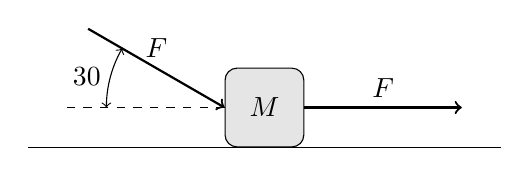
\begin{tikzpicture}
        %% Surface
        \draw (-3,0) -- (3,0);
        %% Block
        \node[draw,fill=white!90!black,rectangle,rounded corners=1ex,minimum size=1cm,anchor=south] (M) at (0,0) {$M$};
        %% Vectors
        \draw[thick,->] (M.east) -- ++(0:2) node[pos=0.5,anchor=south] {$F$};
        \draw[thick,<-] (M.west) -- ++(150:2) node[pos=0.5,anchor=south] {$F$};
        \draw[dashed] (M.west) -- ++(180:2);
        \draw[<->] (M.west) ++(180:1.5) arc (180:150:1.5) node[pos=0.5,anchor=east] {\ang{30}};
    \end{tikzpicture}
    \end{center}
    If $F=\SI{20}{\newton}$ and $M=\SI{5.0}{\kilo\gram}$,
        what is the magnitude of the resulting acceleration of the block?
    \begin{multicols}{3}
    \begin{choices}
        \wrongchoice{\SI{5.3}{\meter\per\second\squared}}
        \wrongchoice{\SI{6.2}{\meter\per\second\squared}}
      \correctchoice{\SI{7.5}{\meter\per\second\squared}}
        \wrongchoice{\SI{4.7}{\meter\per\second\squared}}
        \wrongchoice{\SI{3.2}{\meter\per\second\squared}}
    \end{choices}
    \end{multicols}
\end{question}
}

\element{serway-mc}{
\begin{question}{serway-ch05-q10}
    The only two forces acting on a body have magnitudes of \SI{20}{\newton} and \SI{35}{\newton} and directions that differ by \ang{80}. 
    The resulting acceleration has a magnitude of \SI{20}{\meter\per\second\squared}.
    What is the mass of the body?
    \begin{multicols}{3}
    \begin{choices}
        \wrongchoice{\SI{2.4}{\kilo\gram}}
      \correctchoice{\SI{2.2}{\kilo\gram}}
        \wrongchoice{\SI{2.7}{\kilo\gram}}
        \wrongchoice{\SI{3.1}{\kilo\gram}}
        \wrongchoice{\SI{1.5}{\kilo\gram}}
    \end{choices}
    \end{multicols}
\end{question}
}

\element{serway-mc}{
\begin{question}{serway-ch05-q11}
    If the only forces acting on a \SI{2.0}{\kilo\gram} mass are
        $F_1=\left(3\hat{\imath} - 8\hat{j}\right)\,\si{\newton}$ and
        $F_2=\left(5\hat{\imath} + 3\hat{j}\right)\,\si{\newton}$,
        what is the magnitude of the acceleration of the particle?
    \begin{multicols}{3}
    \begin{choices}
        \wrongchoice{\SI{1.5}{\meter\per\second\squared}}
        \wrongchoice{\SI{6.5}{\meter\per\second\squared}}
      \correctchoice{\SI{4.7}{\meter\per\second\squared}}
        \wrongchoice{\SI{9.4}{\meter\per\second\squared}}
        \wrongchoice{\SI{7.2}{\meter\per\second\squared}}
    \end{choices}
    \end{multicols}
\end{question}
}

\element{serway-mc}{
\begin{question}{serway-ch05-q12}
    At an instant when a \SI{4.0}{\kilo\gram} object has an acceleration equal to $\left(5\hat{\imath} + 3\hat{j}\right)\,\si{\meter\per\second\squared}$,
        one of the two forces acting on the object is known to be $\left(12\hat{\imath} + 22\hat{j}\right)\,\si{\newton}$.
    Determine the magnitude of the other force acting on the object.
    \begin{multicols}{3}
    \begin{choices}
        \wrongchoice{\SI{2.0}{\newton}}
      \correctchoice{\SI{13}{\newton}}
        \wrongchoice{\SI{18}{\newton}}
        \wrongchoice{\SI{1.7}{\newton}}
        \wrongchoice{\SI{20}{\newton}}
    \end{choices}
    \end{multicols}
\end{question}
}

\element{serway-mc}{
\begin{question}{serway-ch05-q13}
    If $F=\SI{4.0}{\newton}$ and $m=\SI{2.0}{\kilo\gram}$,
        what is the magnitude a of the acceleration for the block shown below? 
    \begin{center}
    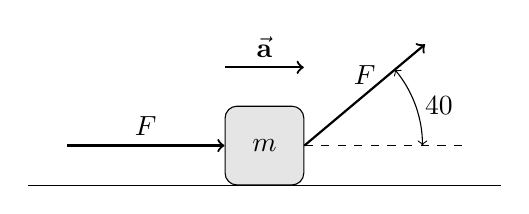
\begin{tikzpicture}
        %% Surface
        \draw (-3,0) -- (3,0);
        %% Block
        \node[draw,fill=white!90!black,rectangle,rounded corners=1ex,minimum size=1cm,anchor=south] (M) at (0,0) {$m$};
        %% ACceleration
        \draw[thick,->] (-0.5,1.5) -- (0.5,1.5) node[pos=0.5,anchor=south] {$\vec{\mathbf{a}}$};
        %% Vectors
        \draw[thick,<-] (M.west) -- ++(180:2) node[pos=0.5,anchor=south] {$F$};
        \draw[thick,->] (M.east) -- ++(40:2) node[pos=0.5,anchor=south] {$F$};
        \draw[dashed] (M.east) -- ++(0:2);
        \draw[<->] (M.east) ++(0:1.5) arc (0:40:1.5) node[pos=0.5,anchor=west] {\ang{40}};
    \end{tikzpicture}
    \end{center}
    The surface is frictionless.
    \begin{multicols}{3}
    \begin{choices}
        \wrongchoice{\SI{5.3}{\meter\per\second\squared}}
        \wrongchoice{\SI{4.4}{\meter\per\second\squared}}
      \correctchoice{\SI{3.5}{\meter\per\second\squared}}
        \wrongchoice{\SI{6.2}{\meter\per\second\squared}}
        \wrongchoice{\SI{8.4}{\meter\per\second\squared}}
    \end{choices}
    \end{multicols}
\end{question}
}

\element{serway-mc}{
\begin{question}{serway-ch05-q14}
    A block is pushed up a frictionless \ang{30} incline by an applied force as shown.
    \begin{center}
    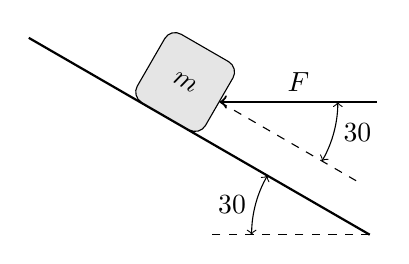
\begin{tikzpicture}
        %% Surface
        \draw[dashed] (0,0) -- (-2,0);
        \draw[thick] (0,0) -- ++ (150:5);
        \draw[<->] (180:1.5) arc (180:150:1.5) node[pos=0.5,anchor=east] {\ang{30}};
        %% Block
        \node[draw,fill=white!90!black,rectangle,rounded corners=1ex,minimum size=1cm,rotate=-30,anchor=south] (M) at (150:3.0) {$m$};
        %% Vectors
        \draw[thick,<-] (M.east) -- ++(0:2) node[pos=0.5,anchor=south] {$F$};
        \draw[dashed] (M.east) -- ++(-30:2);
        \draw[<->] (M.east) ++(-30:1.5) arc (-30:0:1.5) node[pos=0.5,anchor=west] {\ang{30}};
    \end{tikzpicture}
    \end{center}
    If $F=\SI{25}{\newton}$ and $M=\SI{3.0}{\kilo\gram}$,
        what is the magnitude of the resulting acceleration of the block?
    \begin{multicols}{3}
    \begin{choices}
      \correctchoice{\SI{2.3}{\meter\per\second\squared}}
        \wrongchoice{\SI{4.6}{\meter\per\second\squared}}
        \wrongchoice{\SI{3.5}{\meter\per\second\squared}}
        \wrongchoice{\SI{2.9}{\meter\per\second\squared}}
        \wrongchoice{\SI{5.1}{\meter\per\second\squared}}
    \end{choices}
    \end{multicols}
\end{question}
}

\element{serway-mc}{
\begin{question}{serway-ch05-q15}
    A \SI{5.0}{\kilo\gram} object is suspended by a string from the ceiling of an elevator that is accelerating downward at a rate of \SI{2.6}{\meter\per\second\squared}.
    What is the tension in the string?
    \begin{multicols}{3}
    \begin{choices}
        \wrongchoice{\SI{49}{\newton}}
      \correctchoice{\SI{36}{\newton}}
        \wrongchoice{\SI{62}{\newton}}
        \wrongchoice{\SI{13}{\newton}}
        \wrongchoice{\SI{52}{\newton}}
    \end{choices}
    \end{multicols}
\end{question}
}

\element{serway-mc}{
\begin{question}{serway-ch05-q16}
    The tension in a string from which a \SI{4.0}{\kilo\gram} object is suspended in an elevator is equal to \SI{44}{\newton}. 
    What is the acceleration of the elevator?
    \begin{multicols}{2}
    \begin{choices}
        \wrongchoice{\SI{11}{\meter\per\second\squared} upward}
      \correctchoice{\SI{1.2}{\meter\per\second\squared} upward}
        \wrongchoice{\SI{1.2}{\meter\per\second\squared} downward}
        \wrongchoice{\SI{10}{\meter\per\second\squared} upward}
        \wrongchoice{\SI{2.4}{\meter\per\second\squared} downward}
    \end{choices}
    \end{multicols}
\end{question}
}

\element{serway-mc}{
\begin{question}{serway-ch05-q17}
    A \SI{5.0}{\kilo\gram} mass is attached to the ceiling of an elevator by a rope whose mass is negligible. 
    What force does the mass exert on the rope when the elevator has an acceleration of \SI{4.0}{\meter\per\second\squared} upward?
    \begin{multicols}{2}
    \begin{choices}
      \correctchoice{\SI{69}{\newton} downward}
        \wrongchoice{\SI{29}{\newton} downward}
        \wrongchoice{\SI{49}{\newton} downward}
        \wrongchoice{\SI{20}{\newton} downward}
        \wrongchoice{\SI{19}{\newton} downward}
    \end{choices}
    \end{multicols}
\end{question}
}

\element{serway-mc}{
\begin{question}{serway-ch05-q18}
    A \SI{5.0}{\kilo\gram} mass is suspended by a string from the ceiling of an elevator that is moving upward with a speed which is decreasing at a constant rate of \SI{2.0}{\meter\per\second} in each second. 
    What is the tension in the string supporting the mass?
    \begin{multicols}{3}
    \begin{choices}
        \wrongchoice{\SI{49}{\newton}}
      \correctchoice{\SI{39}{\newton}}
        \wrongchoice{\SI{59}{\newton}}
        \wrongchoice{\SI{10}{\newton}}
        \wrongchoice{\SI{42}{\newton}}
    \end{choices}
    \end{multicols}
\end{question}
}

\element{serway-mc}{
\begin{question}{serway-ch05-q19}
    A person weighing \SI{0.70}{\kilo\newton} rides in an elevator that has an upward acceleration of \SI{1.5}{\meter\per\second\squared}. 
    What is the magnitude of the force of the elevator floor on the person?
    \begin{multicols}{3}
    \begin{choices}
        \wrongchoice{\SI{0.11}{\kilo\newton}}
      \correctchoice{\SI{0.81}{\kilo\newton}}
        \wrongchoice{\SI{0.70}{\kilo\newton}}
        \wrongchoice{\SI{0.59}{\kilo\newton}}
        \wrongchoice{\SI{0.64}{\kilo\newton}}
    \end{choices}
    \end{multicols}
\end{question}
}

\element{serway-mc}{
\begin{question}{serway-ch05-q20}
    A \SI{3.0}{\kilo\gram} block slides on a frictionless \ang{20} inclined plane. 
    A force of \SI{16}{\newton} acting parallel to the incline and up the incline is applied to the block. 
    What is the acceleration of the block?
    \begin{choices}
        \wrongchoice{\SI{2.0}{\meter\per\second\squared} down the incline}
        \wrongchoice{\SI{5.3}{\meter\per\second\squared} up the incline}
      \correctchoice{\SI{2.0}{\meter\per\second\squared} up the incline}
        \wrongchoice{\SI{3.9}{\meter\per\second\squared} down the incline}
        \wrongchoice{\SI{3.9}{\meter\per\second\squared} up the incline}
    \end{choices}
\end{question}
}

\element{serway-mc}{
\begin{question}{serway-ch05-q21}
    A \SI{2.0}{\kilo\gram} block slides on a frictionless \ang{25} inclined plane. 
    A force of \SI{4.6}{\newton} acting parallel to the incline and up the incline is applied to the block. 
    What is the acceleration of the block?
    \begin{choices}
        \wrongchoice{\SI{1.8}{\meter\per\second\squared} up the incline}
        \wrongchoice{\SI{2.3}{\meter\per\second\squared} up the incline}
        \wrongchoice{\SI{6.6}{\meter\per\second\squared} down the incline}
      \correctchoice{\SI{1.8}{\meter\per\second\squared} down the incline}
        \wrongchoice{\SI{2.3}{\meter\per\second\squared} down the incline}
    \end{choices}
\end{question}
}

\element{serway-mc}{
\begin{question}{serway-ch05-q22}
    A \SI{2.0}{\kilo\gram} block slides on a frictionless \ang{15} inclined plane. 
    A force acting parallel to the incline is applied to the block. 
    The acceleration of the block is \SI{1.5}{\meter\per\second\squared} down the incline. 
    What is the applied force?
    \begin{choices}
        \wrongchoice{\SI{8.1}{\newton} down the incline}
        \wrongchoice{\SI{3.0}{\newton} down the incline}
      \correctchoice{\SI{2.1}{\newton} up the incline}
        \wrongchoice{\SI{3.0}{\newton} up the incline}
        \wrongchoice{\SI{8.1}{\newton} up the incline}
    \end{choices}
\end{question}
}

\element{serway-mc}{
\begin{question}{serway-ch05-q23}
    A \SI{1.5}{\kilo\gram} object has a velocity of $5\hat{j}\,\si{\meter\per\second}$ at $t = 0$.
    It is accelerated at a constant rate for five seconds after which it has a velocity of $(6\hat{\imath} + 12\hat{j})\,\si{\meter\per\second}$. 
    What is the magnitude of the resultant force acting on the object during this time interval?
    \begin{multicols}{3}
    \begin{choices}
        \wrongchoice{\SI{3.8}{\newton}}
        \wrongchoice{\SI{3.2}{\newton}}
      \correctchoice{\SI{2.8}{\newton}}
        \wrongchoice{\SI{4.3}{\newton}}
        \wrongchoice{\SI{4.6}{\newton}}
    \end{choices}
    \end{multicols}
\end{question}
}

\element{serway-mc}{
\begin{question}{serway-ch05-q24}
    A \SI{1.5}{\kilo\gram} object has a velocity of $5\hat{j}\,\si{\meter\per\second}$ at $t = 0$.
    It is accelerated at a constant rate for five seconds after which it has a velocity of $(6\hat{\imath} + 12\hat{j})\,\si{\meter\per\second}$.
    What is the direction of the resultant force acting on the object during this time interval?
    \begin{multicols}{3}
    \begin{choices}
        \wrongchoice{\ang{65}}
        \wrongchoice{\ang{56}}
        \wrongchoice{\ang{61}}
      \correctchoice{\ang{49}}
        \wrongchoice{\ang{27}}
    \end{choices}
    \end{multicols}
\end{question}
}

\element{serway-mc}{
\begin{question}{serway-ch05-q25}
    A \SI{2.0}{\kilo\gram} object has a velocity of $4.0\hat{\imath}\,\si{\meter\per\second}$ at $t = 0$.
    A constant resultant force of $(2.0\hat{\imath} + 4.0\hat{j})\,\si{\newton}$ then acts on the object for \SI{3.0}{\second}.
    What is the magnitude of the object's velocity at the end of the \SI{3.0}{\second} interval?
    \begin{multicols}{3}
    \begin{choices}
      \correctchoice{\SI{9.2}{\meter\per\second}}
        \wrongchoice{\SI{6.3}{\meter\per\second}}
        \wrongchoice{\SI{8.2}{\meter\per\second}}
        \wrongchoice{\SI{7.2}{\meter\per\second}}
        \wrongchoice{\SI{7.7}{\meter\per\second}}
    \end{choices}
    \end{multicols}
\end{question}
}

\element{serway-mc}{
\begin{question}{serway-ch05-q26}
    A \SI{1.5}{\kilo\gram} mass has an acceleration of
        ${\left(4.0\hat{\imath} - 3.0\hat{j}\right)\,\si{\meter\per\second\squared}}$.
    Only two forces act on the mass. 
    If one of the forces is
        ${\left(2.0\hat{\imath} - 1.4\hat{j}\right)\,\si{\newton}}$,
        what is the magnitude of the other force?
    \begin{multicols}{3}
    \begin{choices}
        \wrongchoice{\SI{4.1}{\newton}}
        \wrongchoice{\SI{6.1}{\newton}}
      \correctchoice{\SI{5.1}{\newton}}
        \wrongchoice{\SI{7.1}{\newton}}
        \wrongchoice{\SI{2.4}{\newton}}
    \end{choices}
    \end{multicols}
\end{question}
}

\element{serway-mc}{
\begin{question}{serway-ch05-q27}
    Only two forces act on a \SI{3.0}{\kilo\gram} mass. 
    One of the forces is \SI{9.0}{\newton} east,
        and the other is \SI{8.0}{\newton} in the direction of \ang{62} north of west. 
    What is the magnitude of the acceleration of the mass?
    \begin{multicols}{3}
    \begin{choices}
        \wrongchoice{\SI{2.0}{\meter\per\second\squared}}
        \wrongchoice{\SI{2.4}{\meter\per\second\squared}}
        \wrongchoice{\SI{3.3}{\meter\per\second\squared}}
      \correctchoice{\SI{2.9}{\meter\per\second\squared}}
        \wrongchoice{\SI{5.7}{\meter\per\second\squared}}
    \end{choices}
    \end{multicols}
\end{question}
}

\element{serway-mc}{
\begin{question}{serway-ch05-q28}
    A book is placed on a chair. 
    Then a videocassette is placed on the book. 
    The floor exerts a normal force
    \begin{choices}
        \wrongchoice{on all three.}
        \wrongchoice{only on the book.}
      \correctchoice{only on the chair.}
        \wrongchoice{upwards on the chair and downwards on the book.}
        \wrongchoice{only on the objects that you have defined to be part of the system.}
    \end{choices}
\end{question}
}

\element{serway-mc}{
\begin{question}{serway-ch05-q29}
    The apparent weight of a fish in an elevator is greatest when the elevator:
    \begin{choices}
        \wrongchoice{moves downward at constant velocity.}
        \wrongchoice{moves upward at constant velocity.}
        \wrongchoice{accelerates downward.}
      \correctchoice{accelerates upward.}
        \wrongchoice{is not moving.}
    \end{choices}
\end{question}
}

\element{serway-mc}{
\begin{question}{serway-ch05-q30}
    The vector sum of three co-planar forces:
    \begin{choices}
        \wrongchoice{must be zero.}
        \wrongchoice{must be perpendicular to one of the three.}
        \wrongchoice{must be parallel to one of the three.}
        \wrongchoice{must be perpendicular to the plane.}
      \correctchoice{may have any direction in the plane.}
    \end{choices}
\end{question}
}

\element{serway-mc}{
\begin{question}{serway-ch05-q31}
    When the vector sum of three co-planar forces, $\mathbf{A}$, $\mathbf{B}$ and $\mathbf{C}$,
        is parallel to $\mathbf{A}$, we can conclude that $\mathbf{B}$ and $\mathbf{C}$:
    \begin{choices}
        \wrongchoice{must sum to zero.}
        \wrongchoice{must be equal and opposite.}
      \correctchoice{must have equal and opposite components perpendicular to $\mathbf{A}$.}
        \wrongchoice{must have equal and opposite components parallel to $\mathbf{A}$.}
        \wrongchoice{must have equal and opposite components parallel and perpendicular to $\mathbf{A}$.}
    \end{choices}
\end{question}
}

\element{serway-mc}{
\begin{question}{serway-ch05-q32}
    A constant force is applied to a body that is already moving. 
    The force is directed at an angle of 60 degrees to the direction of the body's velocity. 
    What is most likely to happen is that
    \begin{choices}
        \wrongchoice{the body will stop moving.}
        \wrongchoice{the body will move in the direction of the force.}
        \wrongchoice{the body's velocity will increase in magnitude but not change direction.}
      \correctchoice{the body will gradually change direction more and more toward that of the force while speeding up.}
        \wrongchoice{the body will first stop moving and then move in the direction of the force.}
    \end{choices}
\end{question}
}

\element{serway-mc}{
\begin{question}{serway-ch05-q33}
    A juggler throws two balls up to the same height so that they pass each other halfway up when $A$ is rising and $B$ is descending. 
    Ignore air resistance and buoyant forces. 
    Which statement is true of the two balls at that point?
    \begin{choices}
        \wrongchoice{There is an residual upward force from the hand on each ball.}
        \wrongchoice{There is a greater residual force from the hand on $A$ than there is on $B$.}
        \wrongchoice{Only gravity acts on $B$ but there is an additional residual force from the hand on $A$.}
        \wrongchoice{There is an additional downwards force besides gravity on each ball.}
      \correctchoice{The only force acting on each ball is the gravitational force.}
    \end{choices}
\end{question}
}

\element{serway-mc}{
\begin{question}{serway-ch05-q34}
    A bumper car is moving at constant velocity when another bumper car starts to push on it with a constant force at an angle of 60 degrees with respect to the first car's initial velocity. 
    The second bumper car continues pushing in exactly that direction for some time. 
    What is most likely to happen is that
    \begin{choices}
        \wrongchoice{the first car will stop moving.}
        \wrongchoice{the first car will move in the direction of the force.}
        \wrongchoice{the first car's velocity will increase in magnitude but not change direction.}
      \correctchoice{the first car's velocity will gradually change direction more and more toward that of the force while increasing in magnitude.}
        \wrongchoice{the first car's velocity will gradually change direction more and more toward that of the force while decreasing in magnitude.}
    \end{choices}
\end{question}
}

\element{serway-mc}{
\begin{question}{serway-ch05-q35}
    You have a machine which can accelerate pucks on frictionless ice. 
    Starting from rest,
        the puck travels a distance $x$ in time $t$ when force $F$ is applied. 
    If force $3F$ is 
        applied, the distance the puck travels in time $t$ is:
    \begin{multicols}{3}
    \begin{choices}
        \wrongchoice{$x$}
        \wrongchoice{$\dfrac{3x}{2}$}
      \correctchoice{$3x$}
        \wrongchoice{$\dfrac{9x}{2}$}
        \wrongchoice{$9x$}
    \end{choices}
    \end{multicols}
\end{question}
}

\element{serway-mc}{
\begin{question}{serway-ch05-q36}
    A constant force $F$ is applied to a body of mass $m$ that initially is headed east at velocity $v_0$ until its velocity becomes $-v_0$. 
    The total time of travel is $2t$. 
    The total distance the body travels in that time is:
    \begin{multicols}{2}
    \begin{choices}
        \wrongchoice{$\dfrac{1}{2}\dfrac{F}{m}t^2$}
      \correctchoice{$\dfrac{F}{m}t^2$}
        \wrongchoice{$v_0t - \dfrac{1}{2}\dfrac{F}{m}t^2$}
        \wrongchoice{$v_0t + \dfrac{1}{2}\dfrac{F}{m}t^2$}
        \wrongchoice{$2\left( v_0t + \dfrac{1}{2}\dfrac{F}{m}t^2\right)$}
    \end{choices}
    \end{multicols}
\end{question}
}

\element{serway-mc}{
\begin{question}{serway-ch05-q37}
    The first of two identical boxes of mass $m$ is sitting on level ground. 
    The second box is sitting on a ramp that makes a \ang{20} angle with the ground. 
    The normal force of the level ground on the first box is $\mathbf{N}_L$;
        the normal force of the ramp on the second box is $\mathbf{N}_R$. 
    Which statement is correct?
    \begin{choices}
        \wrongchoice{$N_R = N_L = mg$}
        \wrongchoice{$N_L = mg$; $N_R = mg\sin\ang{20}.$}
      \correctchoice{$N_L = mg$; $N_R = mg\cos\ang{20}.$}
        \wrongchoice{$N_L = mg$; $N_R = -mg\cos\ang{20}.$}
        \wrongchoice{$N_R = -N_L = -mg$}
    \end{choices}
\end{question}
}

\element{serway-mc}{
\begin{question}{serway-ch05-q38}
    The first of two identical boxes of mass $m$ is sitting on level ground. 
    The second box is sitting on a ramp that makes an angle with the ground. 
    When a force of magnitude $F$ is applied to each box in a direction parallel to the surface it is on,
        upwards on the box on the ramp,
        neither box moves. 
    Which statement comparing the friction force on the box on the level, $f_L$,
        to the friction force on the box on the ramp, $f_R$, is correct?
    \begin{choices}
        \wrongchoice{$f_R = f_L$}
        \wrongchoice{$f_R > f_L$}
      \correctchoice{$f_R < f_L$}
        \wrongchoice{The coefficient of static friction is needed to determine the correct answer.}
        \wrongchoice{The angle between the ramp and the ground is needed to determine the correct answer.}
    \end{choices}
\end{question}
}

\element{serway-mc}{
\begin{question}{serway-ch05-q39}
    The total force needed to drag a box at constant speed across a surface with coefficient of kinetic friction $\mu_k$ is least when the force is applied at an angle $\theta$ such that:
    \begin{multicols}{2}
    \begin{choices}
        \wrongchoice{$\sin\theta = \mu_k$.}
        \wrongchoice{$\cos\theta = \mu_k$.}
        \wrongchoice{$\tan\theta = \mu_k$.}
      \correctchoice{$\cot\theta = \mu_k$.}
        \wrongchoice{$\sec\theta = \mu_k$.}
    \end{choices}
    \end{multicols}
\end{question}
}

\element{serway-mc}{
\begin{question}{serway-ch05-q40}
    A heavy weight is supported by two cables that exert tensions of magnitude $T_1$ and $T_2$.
    \begin{center}
    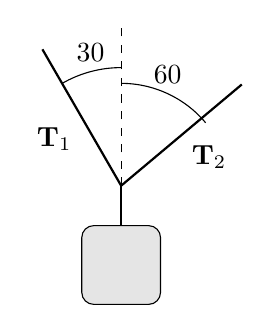
\begin{tikzpicture}
        %% Nodes
        \coordinate (A) at (0,0);
        %% Rope
        \draw[thick] (A) -- ++(40:2) node[pos=0.5,anchor=north west] {$\mathbf{T}_2$};
        \draw[thick] (A) -- ++(120:2) node[pos=0.5,anchor=north east] {$\mathbf{T}_1$};
        \draw[dashed] (A) -- ++(90:2);
        %% Angle
        \draw (A) ++(90:1.5) arc(90:120:1.5) node[pos=0.5,anchor=south] {\ang{30}};
        \draw (A) ++(90:1.3) arc(90:40:1.4) node[pos=0.5,anchor=south] {\ang{60}};
        %% Mass
        \node[draw,fill=white!90!black,rectangle,rounded corners=1ex,minimum size=1cm,anchor=north,yshift=-0.5cm] (M) at (A) {};
        \draw[thick] (M.north) -- (A);
    \end{tikzpicture}
    \end{center}
    Which statement is correct?
    \begin{multicols}{2}
    \begin{choices}
        \wrongchoice{$T_1 = T_2$.}
        \wrongchoice{$T_{1y} = T_{2y}$.}
      \correctchoice{$T_1 > T_2$.}
        \wrongchoice{$T_1 < T_2$.}
        \wrongchoice{We need the mass of the box in order to determine the correct answer.}
    \end{choices}
    \end{multicols}
\end{question}
}

\element{serway-mc}{
\begin{question}{serway-ch05-q41}
    Two people, each of \SI{70}{\kilo\gram} mass, are riding in an elevator. 
    One is standing on the floor. 
    The other is hanging on a rope suspended from the ceiling. 
    Compare the force $F_F$ the floor exerts on the first person to the force $F_R$ the rope exerts on the second person. 
    Which statement is correct?
    \begin{choices}
        \wrongchoice{They are equal and opposite in direction.}
      \correctchoice{The are equal and have the same direction.}
        \wrongchoice{$F_R$ is greater than $F_F$, but they have the same direction.}
        \wrongchoice{$F_R$ is greater than $F_F$, but they have opposite directions.}
        \wrongchoice{$F_R$ is less than $F_F$, but they have the same direction.}
    \end{choices}
\end{question}
}

\element{serway-mc}{
\begin{question}{serway-ch05-q42}
    Two people, each of 70 kg mass, are riding in an elevator. 
    One is standing on the floor. 
    The other is hanging on a rope suspended from the ceiling. 
    Compare the acceleration $a_F$ of the first person to the acceleration $a_R$ of the second person.
    Which statement is correct?
    \begin{choices}
        \wrongchoice{They are equal and opposite in direction.}
      \correctchoice{The are equal and have the same direction.}
        \wrongchoice{The acceleration $a_R$ is greater than $a_F$ , but they have the same direction.}
        \wrongchoice{The acceleration $a_R$ is greater than $a_F$ , but they have opposite directions.}
        \wrongchoice{The acceleration $a_R$ is less than $a_F$ , but they have the same direction.}
    \end{choices}
\end{question}
}

\element{serway-mc}{
\begin{question}{serway-ch05-q43}
    The horizontal surface on which the objects slide is frictionless. 
    \begin{center}
    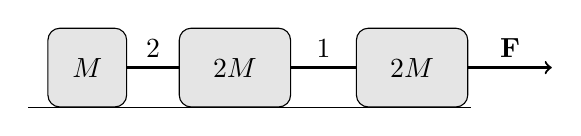
\begin{tikzpicture}[scale=0.75]
        %% Floor
        \draw (-1,0) -- (6.5,0);
        %% Mass
        \node[draw,fill=white!90!black,rectangle,rounded corners=1ex,minimum size=1cm,anchor=south] (A) at (0,0) {$M$};
        \node[draw,fill=white!90!black,rectangle,rounded corners=1ex,minimum width=1.414cm,minimum height=1cm,anchor=south] (B) at (2.5,0) {$2M$};
        \node[draw,fill=white!90!black,rectangle,rounded corners=1ex,minimum width=1.414cm,minimum height=1cm,anchor=south] (C) at (5.5,0) {$2M$};
        %% Rope
        \draw[thick] (A.east) -- (B.west) node[pos=0.5,anchor=south] {2};
        \draw[thick] (B.east) -- (C.west) node[pos=0.5,anchor=south] {1};
        \draw[thick,->] (C.east) -- ++(0:1.414) node[pos=0.5,anchor=south] {$\mathbf{F}$};
    \end{tikzpicture}
    \end{center}
    If $M = \SI{2.0}{\kilo\gram}$,
        the tension in string 1 is \SI{12}{\newton}. 
    Determine $F$.
    \begin{multicols}{3}
    \begin{choices}
        \wrongchoice{\SI{25}{\newton}}
      \correctchoice{\SI{20}{\newton}}
        \wrongchoice{\SI{30}{\newton}}
        \wrongchoice{\SI{35}{\newton}}
        \wrongchoice{\SI{40}{\newton}}
    \end{choices}
    \end{multicols}
\end{question}
}

\element{serway-mc}{
\begin{question}{serway-ch05-q44}
    The horizontal surface on which the objects slide is frictionless. 
    \begin{center}
    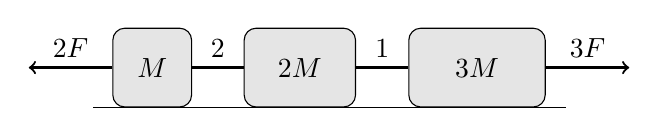
\begin{tikzpicture}[scale=0.75]
        %% Floor
        \draw (-1,0) -- (7,0);
        %% Mass
        \node[draw,fill=white!90!black,rectangle,rounded corners=1ex,minimum size=1cm,anchor=south] (A) at (0,0) {$M$};
        \node[draw,fill=white!90!black,rectangle,rounded corners=1ex,minimum width=1.414cm,minimum height=1cm,anchor=south] (B) at (2.5,0) {$2M$};
        \node[draw,fill=white!90!black,rectangle,rounded corners=1ex,minimum width=1.732cm,minimum height=1cm,anchor=south] (C) at (5.5,0) {$3M$};
        %% Rope
        \draw[thick,->] (A.west) -- ++(180:1.414) node[pos=0.5,anchor=south] {$2F$};
        \draw[thick] (A.east) -- (B.west) node[pos=0.5,anchor=south] {2};
        \draw[thick] (B.east) -- (C.west) node[pos=0.5,anchor=south] {1};
        \draw[thick,->] (C.east) -- ++(0:1.414) node[pos=0.5,anchor=south] {$3F$};
    \end{tikzpicture}
    \end{center}
    If $F=\SI{12}{\newton}$, what is the tension in string 1?
    \begin{multicols}{3}
    \begin{choices}
        \wrongchoice{\SI{35}{\newton}}
      \correctchoice{\SI{30}{\newton}}
        \wrongchoice{\SI{40}{\newton}}
        \wrongchoice{\SI{45}{\newton}}
        \wrongchoice{\SI{25}{\newton}}
    \end{choices}
    \end{multicols}
\end{question}
}

\element{serway-mc}{
\begin{question}{serway-ch05-q45}
    The surface of the inclined plane shown is frictionless. 
    \begin{center}
    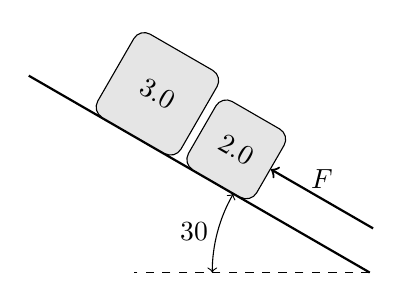
\begin{tikzpicture}
        %% Surface
        \draw[dashed] (0,0) -- (-3,0);
        \draw[thick] (0,0) -- ++ (150:5);
        \draw[<->] (180:2.0) arc (180:150:2.0) node[pos=0.5,anchor=east] {\ang{30}};
        %% Blocks
        \node[draw,fill=white!90!black,rectangle,rounded corners=1ex,minimum size=1.00cm,rotate=-30,anchor=south] (M) at (150:2.25) {\SI{2.0}{\kilo\gram}};
        \node[draw,fill=white!90!black,rectangle,rounded corners=1ex,minimum size=1.22cm,rotate=-30,anchor=south] (N) at (150:3.47) {\SI{3.0}{\kilo\gram}};
        %% Vectors
        \draw[thick,<-] (M.east) -- ++(-30:1.5) node[pos=0.5,anchor=south] {$F$};
    \end{tikzpicture}
    \end{center}
    If $F=\SI{30}{\newton}$,
        what is the magnitude of the force exerted on the \SI{3.0}{\kilo\gram} block by the \SI{2.0}{\kilo\gram} block?
    \begin{multicols}{3}
    \begin{choices}
      \correctchoice{\SI{18}{\newton}}
        \wrongchoice{\SI{27}{\newton}}
        \wrongchoice{\SI{24}{\newton}}
        \wrongchoice{\SI{21}{\newton}}
        \wrongchoice{\SI{15}{\newton}}
    \end{choices}
    \end{multicols}
\end{question}
}

\element{serway-mc}{
\begin{question}{serway-ch05-q46}
    If $P=\SI{6.0}{\newton}$,
        what is the magnitude of the force exerted on block 1 by block 2?
    \begin{center}
    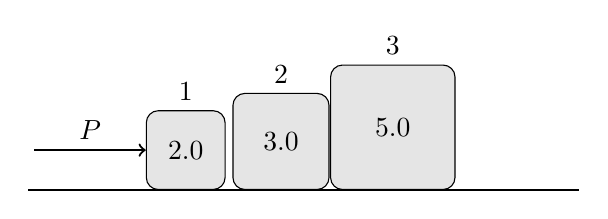
\begin{tikzpicture}
        %% Floor
        \draw (-2,0) -- (5,0);
        %% Mass
        \node[draw,fill=white!90!black,rectangle,rounded corners=1ex,minimum size=1cm,anchor=south] (A) at (0,0) {\SI{2.0}{\kilo\gram}};
        \node[draw,fill=white!90!black,rectangle,rounded corners=1ex,minimum size=1.22cm,anchor=south] (B) at (1.21,0) {\SI{3.0}{\kilo\gram}};
        \node[draw,fill=white!90!black,rectangle,rounded corners=1ex,minimum size=1.58cm,anchor=south] (C) at (2.63,0) {\SI{5.0}{\kilo\gram}};
        %% Labels
        \node[anchor=south] at (A.north) {1};
        \node[anchor=south] at (B.north) {2};
        \node[anchor=south] at (C.north) {3};
        %% Force
        \draw[thick,<-] (A.west) -- ++(180:1.414) node[pos=0.5,anchor=south] {$P$};
    \end{tikzpicture}
    \end{center}
    \begin{multicols}{3}
    \begin{choices}
        \wrongchoice{\SI{6.4}{\newton}}
        \wrongchoice{\SI{5.6}{\newton}}
      \correctchoice{\SI{4.8}{\newton}}
        \wrongchoice{\SI{7.2}{\newton}}
        \wrongchoice{\SI{8.4}{\newton}}
    \end{choices}
    \end{multicols}
\end{question}
}

\element{serway-mc}{
\begin{question}{serway-ch05-q47}
    If $F=\SI{5.0}{\newton}$,
        what is the magnitude of the force exerted by block 2 on block 1?
    \begin{center}
    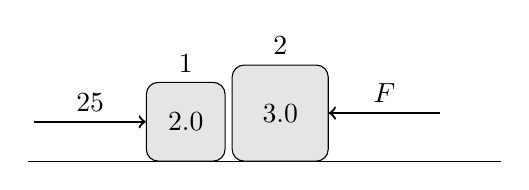
\begin{tikzpicture}
        %% Floor
        \draw (-2,0) -- (4,0);
        %% Mass
        \node[draw,fill=white!90!black,rectangle,rounded corners=1ex,minimum size=1cm,anchor=south] (A) at (0,0) {\SI{2.0}{\kilo\gram}};
        \node[draw,fill=white!90!black,rectangle,rounded corners=1ex,minimum size=1.22cm,anchor=south] (B) at (1.20,0) {\SI{3.0}{\kilo\gram}};
        \node[anchor=south] at (A.north) {1};
        \node[anchor=south] at (B.north) {2};
        %% Force
        \draw[thick,<-] (A.west) -- ++(180:1.414) node[pos=0.5,anchor=south] {\SI{25}{\newton}};
        \draw[thick,<-] (B.east) -- ++(0:1.414) node[pos=0.5,anchor=south] {$F$};
    \end{tikzpicture}
    \end{center}
    \begin{multicols}{3}
    \begin{choices}
      \correctchoice{\SI{17}{\newton}}
        \wrongchoice{\SI{19}{\newton}}
        \wrongchoice{\SI{21}{\newton}}
        \wrongchoice{\SI{23}{\newton}}
        \wrongchoice{\SI{5.0}{\newton}}
    \end{choices}
    \end{multicols}
\end{question}
}

\element{serway-mc}{
\begin{question}{serway-ch05-q48}
    An astronaut who weighs \SI{800}{\newton} on the surface of the earth lifts off from planet Zuton in a space ship. 
    The free-fall acceleration on Zuton is \SI{3.0}{\meter\per\second\squared} (down). 
    At the moment of liftoff the acceleration of the space ship is \SI{0.50}{\meter\per\second\squared} (up). 
    What is the magnitude of the force of the space ship on the astronaut?
    \begin{multicols}{3}
    \begin{choices}
        \wrongchoice{\SI{41}{\kilo\newton}}
      \correctchoice{\SI{0.29}{\kilo\newton}}
        \wrongchoice{\SI{0.24}{\kilo\newton}}
        \wrongchoice{\SI{0.20}{\kilo\newton}}
        \wrongchoice{\SI{0.37}{\kilo\newton}}
    \end{choices}
    \end{multicols}
\end{question}
}

\element{serway-mc}{
\begin{question}{serway-ch05-q49}
    The horizontal surface on which the objects slide is frictionless. 
    \begin{center}
    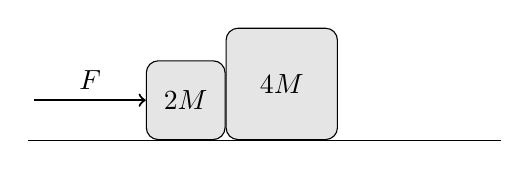
\begin{tikzpicture}
        %% Floor
        \draw (-2,0) -- (4,0);
        %% Mass
        \node[draw,fill=white!90!black,rectangle,rounded corners=1ex,minimum size=1cm,anchor=south] (A) at (0,0) {$2M$};
        \node[draw,fill=white!90!black,rectangle,rounded corners=1ex,minimum size=1.414cm,anchor=south] (B) at (1.22,0) {$4M$};
        %% Force
        \draw[thick,<-] (A.west) -- ++(180:1.414) node[pos=0.5,anchor=south] {$F$};
        %\draw[thick,<-] (B.east) -- ++(0:1.414) node[pos=0.5,anchor=south] {$F$};
    \end{tikzpicture}
    \end{center}
    If $M=\SI{1.0}{\kilo\gram}$ and the magnitude of the force of the   
        small block on the large block is \SI{5.2}{\newton}, determine $F$.
    \begin{multicols}{3}
    \begin{choices}
        \wrongchoice{\SI{6.0}{\newton}}
        \wrongchoice{\SI{9.0}{\newton}}
      \correctchoice{\SI{7.8}{\newton}}
        \wrongchoice{\SI{4.8}{\newton}}
        \wrongchoice{\SI{4.1}{\newton}}
    \end{choices}
    \end{multicols}
\end{question}
}

\element{serway-mc}{
\begin{question}{serway-ch05-q50}
    The horizontal surface on which the objects slide is frictionless. 
    \begin{center}
    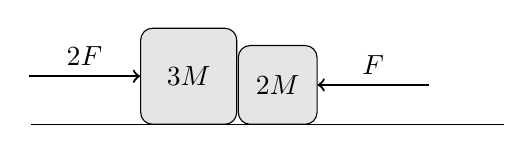
\begin{tikzpicture}
        %% Floor
        \draw (-2,0) -- (4,0);
        %% Mass
        \node[draw,fill=white!90!black,rectangle,rounded corners=1ex,minimum size=1.22cm,anchor=south] (A) at (0,0) {$3M$};
        \node[draw,fill=white!90!black,rectangle,rounded corners=1ex,minimum size=1.00cm,anchor=south] (B) at (1.13,0) {$2M$};
        %% Force
        \draw[thick,<-] (A.west) -- ++(180:1.414) node[pos=0.5,anchor=south] {$2F$};
        \draw[thick,<-] (B.east) -- ++(0:1.414) node[pos=0.5,anchor=south] {$F$};
    \end{tikzpicture}
    \end{center}
    If $F=\SI{6.0}{\newton}$ and $M=\SI{1.0}{\kilo\gram}$,
        what is the magnitude of the force exerted on the large block by the small block?
    \begin{multicols}{3}
    \begin{choices}
        \wrongchoice{\SI{7.7}{\newton}}
        \wrongchoice{\SI{9.8}{\newton}}
        \wrongchoice{\SI{9.1}{\newton}}
      \correctchoice{\SI{8.4}{\newton}}
        \wrongchoice{\SI{6.5}{\newton}}
    \end{choices}
    \end{multicols}
\end{question}
}

\element{serway-mc}{
\begin{question}{serway-ch05-q51}
    A \SI{6.0}{\kilo\gram} object is suspended by a vertical string from the
        ceiling of an elevator which is accelerating upward at a rate of
        \SI{1.8}{\meter\per\second\squared}. 
    Determine the tension in the string.
    \begin{multicols}{3}
    \begin{choices}
        \wrongchoice{\SI{11}{\newton}}
      \correctchoice{\SI{70}{\newton}}
        \wrongchoice{\SI{48}{\newton}}
        \wrongchoice{\SI{59}{\newton}}
        \wrongchoice{\SI{62}{\newton}}
    \end{choices}
    \end{multicols}
\end{question}
}

\element{serway-mc}{
\begin{question}{serway-ch05-q52}
    An \SI{8.0}{\kilo\gram} object rests on the floor of an elevator which is accelerating downward at a rate of \SI{1.3}{\meter\per\second\squared}. 
    What is the magnitude of the force the object exerts on the floor of the elevator?
    \begin{multicols}{3}
    \begin{choices}
        \wrongchoice{\SI{59}{\newton}}
        \wrongchoice{\SI{10}{\newton}}
        \wrongchoice{\SI{89}{\newton}}
      \correctchoice{\SI{68}{\newton}}
        \wrongchoice{\SI{78}{\newton}}
    \end{choices}
    \end{multicols}
\end{question}
}

\element{serway-mc}{
\begin{question}{serway-ch05-q53}
    A \SI{70}{\kilo\gram} stunt artist rides in a rocket sled which slides along a flat inclined surface. 
    At an instant when the sled’s acceleration has a horizontal component of \SI{6.0}{\meter\per\second\squared} and a downward component of \SI{2.8}{\meter\per\second\squared},
        what is the magnitude of the force on the rider by the sled?
    \begin{multicols}{3}
    \begin{choices}
        \wrongchoice{\SI{0.83}{\kilo\newton}}
        \wrongchoice{\SI{0.98}{\kilo\newton}}
      \correctchoice{\SI{0.65}{\kilo\newton}}
        \wrongchoice{\SI{0.68}{\kilo\newton}}
        \wrongchoice{\SI{0.72}{\kilo\newton}}
    \end{choices}
    \end{multicols}
\end{question}
}

\element{serway-mc}{
\begin{question}{serway-ch05-q54}
    If $F=\SI{40}{\newton}$ and $M=\SI{1.5}{\kilo\gram}$,
        what is the tension in the string connecting $M$ and $2M$?
    Assume that all surfaces are frictionless.
    \begin{center}
    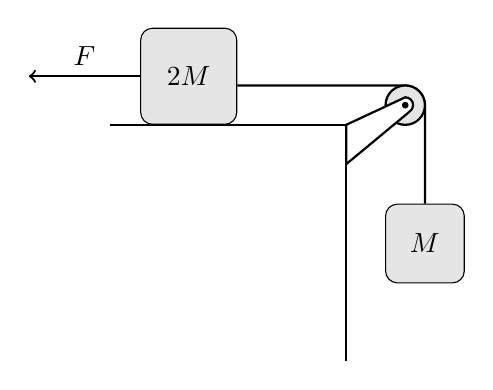
\begin{tikzpicture}
        %% Floor
        \draw[thick] (-3,0) -- (0,0) -- (0,-3);
        %% Mass
        \node[draw,fill=white!90!black,rectangle,rounded corners=1ex,minimum size=1.22cm,anchor=south] (A) at (-2,0) {$2M$};
        \node[draw,fill=white!90!black,rectangle,rounded corners=1ex,minimum size=1.00cm,anchor=north] (B) at (1,-1) {$M$};
        %% Rope and Pulley
        \draw[thick] (A.south east) ++(90:0.5) -- (0.75,0.5) arc(90:0:0.25) -- (B.north);
        \draw[thick,fill=white!90!black] (0.75,0.25) circle (0.25); 
        \draw[thick,fill=white] (0,0) -- (0.75,0.35) arc (90:-60:0.1) -- (0,-0.5) -- cycle;
        \draw[fill] (0.75,0.25) circle (1pt);
        %% Force
        \draw[thick,->] (A.west) -- ++(180:1.414) node[pos=0.5,anchor=south] {$F$};
    \end{tikzpicture}
    \end{center}
    \begin{multicols}{3}
    \begin{choices}
        \wrongchoice{\SI{13}{\newton}}
      \correctchoice{\SI{23}{\newton}}
        \wrongchoice{\SI{36}{\newton}}
        \wrongchoice{\SI{15}{\newton}}
        \wrongchoice{\SI{28}{\newton}}
    \end{choices}
    \end{multicols}
\end{question}
}

\element{serway-mc}{
\begin{question}{serway-ch05-q55}
    The system shown is released from rest and moves \SI{50}{\centi\meter} in \SI{1.0}{\second}.
    What is the value of $M$? 
    All surfaces are frictionless.
    \begin{center}
    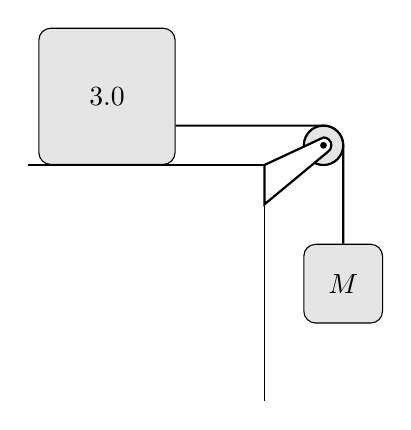
\begin{tikzpicture}
        %% Floor
        \draw (-3,0) -- (0,0) -- (0,-3);
        %% Mass
        \node[draw,fill=white!90!black,rectangle,rounded corners=1ex,minimum size=1.73cm,anchor=south] (A) at (-2,0) {\SI{3.0}{\kilo\gram}};
        \node[draw,fill=white!90!black,rectangle,rounded corners=1ex,minimum size=1.00cm,anchor=north] (B) at (1,-1) {$M$};
        %% Rope and Pulley
        \draw[thick] (A.south east) ++(90:0.5) -- (0.75,0.5) arc(90:0:0.25) -- (B.north);
        \draw[thick,fill=white!90!black] (0.75,0.25) circle (0.25); 
        \draw[thick,fill=white] (0,0) -- (0.75,0.35) arc (90:-60:0.1) -- (0,-0.5) -- cycle;
        \draw[fill] (0.75,0.25) circle (1pt);
    \end{tikzpicture}
    \end{center}
    \begin{multicols}{3}
    \begin{choices}
        \wrongchoice{\SI{0.42}{\kilo\gram}}
      \correctchoice{\SI{0.34}{\kilo\gram}}
        \wrongchoice{\SI{0.50}{\kilo\gram}}
        \wrongchoice{\SI{0.59}{\kilo\gram}}
        \wrongchoice{\SI{0.68}{\kilo\gram}}
    \end{choices}
    \end{multicols}
\end{question}
}

\element{serway-mc}{
\begin{question}{serway-ch05-q56}
    If $F=\SI{40}{\newton}$ and $M=\SI{2.0}{\kilo\gram}$,
        what is the magnitude of the acceleration of the suspended object? 
    All surfaces are frictionless.
    \begin{center}
    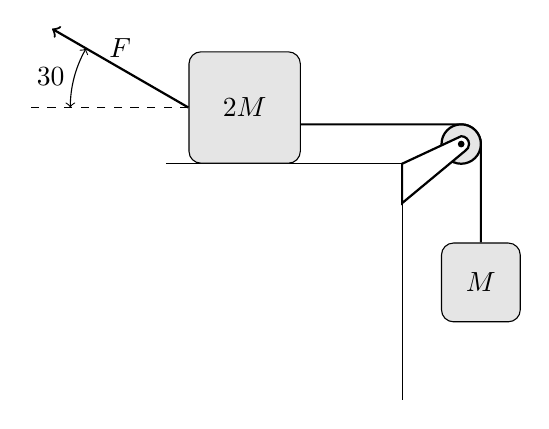
\begin{tikzpicture}
        %% Floor
        \draw (-3,0) -- (0,0) -- (0,-3);
        %% Mass
        \node[draw,fill=white!90!black,rectangle,rounded corners=1ex,minimum size=1.414cm,anchor=south] (A) at (-2,0) {$2M$};
        \node[draw,fill=white!90!black,rectangle,rounded corners=1ex,minimum size=1.00cm,anchor=north] (B) at (1,-1) {$M$};
        %% Rope and Pulley
        \draw[thick] (A.south east) ++(90:0.5) -- (0.75,0.5) arc(90:0:0.25) -- (B.north);
        \draw[thick,fill=white!90!black] (0.75,0.25) circle (0.25); 
        \draw[thick,fill=white] (0,0) -- (0.75,0.35) arc (90:-60:0.1) -- (0,-0.5) -- cycle;
        \draw[fill] (0.75,0.25) circle (1pt);
        %% Force
        \draw[dashed] (A.west) -- ++(180:2);
        \draw[<->] (A.west) ++ (180:1.5) arc(180:150:1.5) node[pos=0.5,anchor=east] {\ang{30}};
        \draw[thick,->] (A.west) -- ++(150:2) node[pos=0.5,anchor=south] {$F$};
    \end{tikzpicture}
    \end{center}
    \begin{multicols}{3}
    \begin{choices}
        \wrongchoice{\SI{1.2}{\meter\per\second\squared}}
        \wrongchoice{\SI{2.0}{\meter\per\second\squared}}
        \wrongchoice{\SI{1.5}{\meter\per\second\squared}}
      \correctchoice{\SI{2.5}{\meter\per\second\squared}}
        \wrongchoice{\SI{5.6}{\meter\per\second\squared}}
    \end{choices}
    \end{multicols}
\end{question}
}

\element{serway-mc}{
\begin{question}{serway-ch05-q57}
    If $M=\SI{2.2}{\kilo\gram}$,
        what is the tension in the connecting string? 
    The pulley and all surfaces are frictionless.
    \begin{center}
    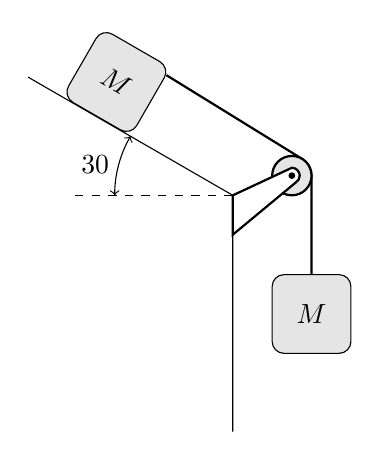
\begin{tikzpicture}
        %% Floor
        \draw (150:3) -- (0,0) -- (0,-3);
        \draw[dashed] (0,0) -- (-2,0);
        \draw[<->] (180:1.5) arc (180:150:1.5) node[pos=0.5,anchor=east] {\ang{30}};
        %% Mass
        \node[draw,fill=white!90!black,rectangle,rounded corners=1ex,minimum size=1cm,rotate=-30,anchor=south] (A) at (150:2) {$M$};
        \node[draw,fill=white!90!black,rectangle,rounded corners=1ex,minimum size=1cm,anchor=north] (B) at (1,-1) {$M$};
        %% Rope and Pulley
        \draw[thick] (A.south east) ++(60:0.9) -- (0.875,0.466) arc(60:0:0.25) -- (B.north);
        \draw[thick,fill=white!90!black] (0.75,0.25) circle (0.25); 
        \draw[thick,fill=white] (0,0) -- (0.75,0.35) arc (90:-60:0.1) -- (0,-0.5) -- cycle;
        \draw[fill] (0.75,0.25) circle (1pt);
    \end{tikzpicture}
    \end{center}
    \begin{multicols}{3}
    \begin{choices}
        \wrongchoice{\SI{6.4}{\newton}}
        \wrongchoice{\SI{5.9}{\newton}}
      \correctchoice{\SI{5.4}{\newton}}
        \wrongchoice{\SI{6.9}{\newton}}
        \wrongchoice{\SI{8.3}{\newton}}
    \end{choices}
    \end{multicols}
\end{question}
}

\element{serway-mc}{
\begin{question}{serway-ch05-q58}
    A \SI{5.0}{\kilo\gram} mass sits on the floor of an elevator that has a downward acceleration of \SI{1.0}{\meter\per\second\squared}.
    On top of the \SI{5.0}{\kilo\gram} mass is an object of unknown mass. 
    The force of the elevator on the \SI{5.0}{\kilo\gram} mass is \SI{80}{\newton} up. 
    Determine the unknown mass.
    \begin{multicols}{3}
    \begin{choices}
        \wrongchoice{\SI{3.3}{\kilo\gram}}
        \wrongchoice{\SI{2.4}{\kilo\gram}}
        \wrongchoice{\SI{1.6}{\kilo\gram}}
      \correctchoice{\SI{4.1}{\kilo\gram}}
        \wrongchoice{\SI{5.0}{\kilo\gram}}
    \end{choices}
    \end{multicols}
\end{question}
}

\element{serway-mc}{
\begin{question}{serway-ch05-q59}
    If the tension, $T$, is \SI{15}{\newton} and the magnitude of the acceleration,
        $a$, is \SI{3.0}{\meter\per\second\squared}, what is the mass, $m$,
        of the suspended object? 
    \begin{center}
    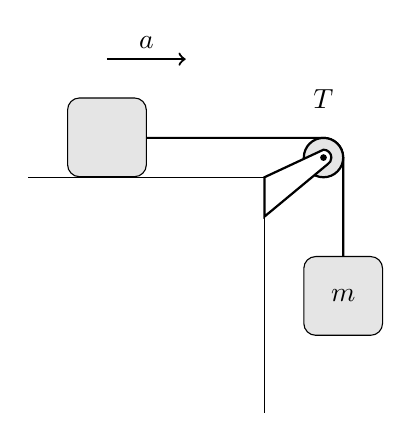
\begin{tikzpicture}
        %% Floor
        \draw (-3,0) -- (0,0) -- (0,-3);
        %% Mass
        \node[draw,fill=white!90!black,rectangle,rounded corners=1ex,minimum size=1.0cm,anchor=south] (A) at (-2,0) {};
        \node[draw,fill=white!90!black,rectangle,rounded corners=1ex,minimum size=1.0cm,anchor=north] (B) at (1,-1) {$m$};
        %% Labels
        \draw[thick,->] (-2,1.5) -- ++ (0:1) node[pos=0.5,anchor=south] {$a$};
        \node[anchor=south] at (0.75,0.75) {$T$};
        %% Rope and Pully
        \draw[thick] (A.south east) ++(90:0.5) -- (0.75,0.5) arc(90:0:0.25) -- (B.north);
        \draw[thick,fill=white!90!black] (0.75,0.25) circle (0.25); 
        \draw[thick,fill=white] (0,0) -- (0.75,0.35) arc (90:-60:0.1) -- (0,-0.5) -- cycle;
        \draw[fill] (0.75,0.25) circle (1pt);
    \end{tikzpicture}
    \end{center}
    Assume that all surfaces and the pulley are frictionless?
    \begin{multicols}{3}
    \begin{choices}
        \wrongchoice{\SI{3.1}{\kilo\gram}}
        \wrongchoice{\SI{2.5}{\kilo\gram}}
        \wrongchoice{\SI{2.8}{\kilo\gram}}
      \correctchoice{\SI{2.2}{\kilo\gram}}
        \wrongchoice{\SI{3.7}{\kilo\gram}}
    \end{choices}
    \end{multicols}
\end{question}
}

\element{serway-mc}{
\begin{question}{serway-ch05-q60}
    If $F=\SI{8.0}{\newton}$ and $M=\SI{1.0}{\kilo\gram}$,
        what is the tension in the connecting string? 
    \begin{center}
    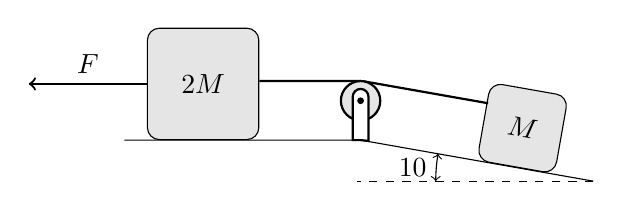
\begin{tikzpicture}
        %% Floor
        \draw (-3,0) -- (0,0) -- ++(350:3);
        \draw[dashed] (350:3) -- ++(180:3);
        \draw[<->] (350:3) ++(180:2) arc (180:170:2) node[pos=0.5,anchor=east] {\ang{10}};
        %% Mass
        \node[draw,fill=white!90!black,rectangle,rounded corners=1ex,minimum size=1.414cm,anchor=south] (A) at (-2,0) {$2M$};
        \node[draw,fill=white!90!black,rectangle,rounded corners=1ex,minimum size=1.0cm,anchor=south,rotate=-10] (B) at (350:2) {$M$};
        %% Rope and Pully
        \draw[thick] (A.south east) ++(90:0.75) -- (0,0.75) arc(90:80:0.25) -- ++(350:1.6);
        \draw[thick,fill=white!90!black] (0,0.5) circle (0.25); 
        \draw[thick,fill=white] (-0.1,0) -- (-0.1,0.55) arc (180:0:0.1) -- (0.1,-0.01) -- (0,0) -- cycle;
        \draw[fill] (0,0.50) circle (1pt);
        %% Forces
        \draw[thick,->] (A.west) -- ++(180:1.5) node[pos=0.5,anchor=south] {$F$};
    \end{tikzpicture}
    \end{center}
    The pulley and all surfaces are frictionless.
    \begin{multicols}{3}
    \begin{choices}
        \wrongchoice{\SI{4.1}{\newton}}
        \wrongchoice{\SI{3.5}{\newton}}
      \correctchoice{\SI{3.8}{\newton}}
        \wrongchoice{\SI{3.1}{\newton}}
        \wrongchoice{\SI{4.8}{\newton}}
    \end{choices}
    \end{multicols}
\end{question}
}

\element{serway-mc}{
\begin{question}{serway-ch05-q61}
    In the figure, if $F=\SI{2.0}{\newton}$ and $M=\SI{1.0}{\kilo\gram}$,
        what is the tension in the connecting string? 
    \begin{center}
    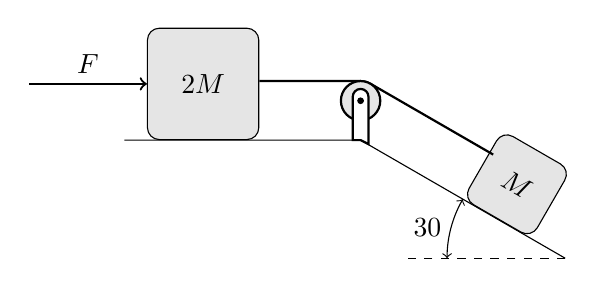
\begin{tikzpicture}
        %% Floor
        \draw (-3,0) -- (0,0) -- ++(330:3);
        \draw[dashed] (330:3) -- ++(180:2);
        \draw[<->] (330:3) ++(180:1.5) arc (180:150:1.5) node[pos=0.5,anchor=east] {\ang{30}};
        %% Mass
        \node[draw,fill=white!90!black,rectangle,rounded corners=1ex,minimum size=1.414cm,anchor=south] (A) at (-2,0) {$2M$};
        \node[draw,fill=white!90!black,rectangle,rounded corners=1ex,minimum size=1.0cm,anchor=south,rotate=-30] (B) at (330:2) {$M$};
        %% Rope and Pully
        \draw[thick] (A.south east) ++(90:0.75) -- (0,0.75) arc(90:60:0.25) -- ++(330:1.8);
        \draw[thick,fill=white!90!black] (0,0.5) circle (0.25); 
        \draw[thick,fill=white] (-0.1,0) -- (-0.1,0.55) arc (180:0:0.1) -- (0.1,-0.05) -- (0,0) -- cycle;
        \draw[fill] (0,0.50) circle (1pt);
        %% Forces
        \draw[thick,<-] (A.west) -- ++(180:1.5) node[pos=0.5,anchor=south] {$F$};
    \end{tikzpicture}
    \end{center}
    The pulley and all surfaces are frictionless.
    \begin{multicols}{3}
    \begin{choices}
      \correctchoice{\SI{2.6}{\newton}}
        \wrongchoice{\SI{1.1}{\newton}}
        \wrongchoice{\SI{2.1}{\newton}}
        \wrongchoice{\SI{1.6}{\newton}}
        \wrongchoice{\SI{3.7}{\newton}}
    \end{choices}
    \end{multicols}
\end{question}
}

\element{serway-mc}{
\begin{question}{serway-ch05-q62}
    A \SI{4.0}{\kilo\gram} block slides down a \ang{35} incline at a constant speed when a \SI{16}{\newton} force is applied acting up and parallel to the incline. 
    What is the coefficient of kinetic friction between the block and the surface of the incline?
    \begin{multicols}{3}
    \begin{choices}
      \correctchoice{\num{0.20}}
        \wrongchoice{\num{0.23}}
        \wrongchoice{\num{0.26}}
        \wrongchoice{\num{0.33}}
        \wrongchoice{\num{0.41}}
    \end{choices}
    \end{multicols}
\end{question}
}

\element{serway-mc}{
\begin{question}{serway-ch05-q63}
    A block is pushed across a horizontal surface by the force shown. 
    \begin{center}
    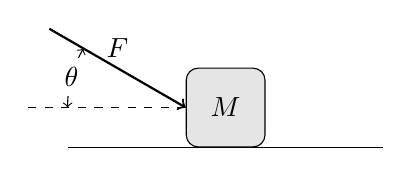
\begin{tikzpicture}
        %% Floor
        \draw (-2,0) -- (2,0);
        %% Mass
        \node[draw,fill=white!90!black,rectangle,rounded corners=1ex,minimum size=1cm,anchor=south] (A) at (0,0) {$M$};
        %% Forces
        \draw[dashed] (A.west) -- ++(180:2);
        \draw[<->] (A.west) ++ (180:1.5) arc (180:150:1.5) node[pos=0.5,anchor=center,fill=white] {$\theta$};
        \draw[thick,<-] (A.west) -- ++(150:2) node[pos=0.5,anchor=south] {$F$};
    \end{tikzpicture}
    \end{center}
    If the coefficient of kinetic friction between the block and the surface is \num{0.30},
        $F=\SI{20}{\newton}$, $\theta=\ang{30}$, and $M=\SI{3.0}{\kilo\gram}$,
        what is the magnitude of the acceleration of the block?
    \begin{multicols}{3}
    \begin{choices}
        \wrongchoice{\SI{2.8}{\meter\per\second\squared}}
        \wrongchoice{\SI{2.3}{\meter\per\second\squared}}
      \correctchoice{\SI{1.8}{\meter\per\second\squared}}
        \wrongchoice{\SI{3.3}{\meter\per\second\squared}}
        \wrongchoice{\SI{5.4}{\meter\per\second\squared}}
    \end{choices}
    \end{multicols}
\end{question}
}

\element{serway-mc}{
\begin{question}{serway-ch05-q64}
    A \SI{3.0}{\kilo\gram} block moves up a \ang{40} incline with constant speed under the action of a \SI{26}{\newton} force acting up and parallel to the incline. 
    What magnitude force must act up and parallel to the incline for the block to move down the incline at constant velocity?
    \begin{multicols}{3}
    \begin{choices}
        \wrongchoice{\SI{14}{\newton}}
      \correctchoice{\SI{12}{\newton}}
        \wrongchoice{\SI{16}{\newton}}
        \wrongchoice{\SI{18}{\newton}}
        \wrongchoice{\SI{25}{\newton}}
    \end{choices}
    \end{multicols}
\end{question}
}

\element{serway-mc}{
\begin{question}{serway-ch05-q65}
    The block shown is pulled across the horizontal surface at a constant speed by the force shown. 
    \begin{center}
    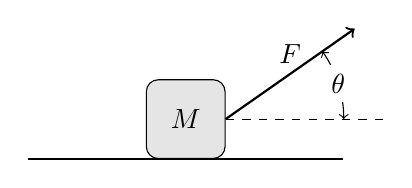
\begin{tikzpicture}
        %% Floor
        \draw (-2,0) -- (2,0);
        %% Mass
        \node[draw,fill=white!90!black,rectangle,rounded corners=1ex,minimum size=1cm,anchor=south] (A) at (0,0) {$M$};
        %% Forces
        \draw[dashed] (A.east) -- ++(0:2);
        \draw[<->] (A.east) ++ (0:1.5) arc (0:35:1.5) node[pos=0.5,anchor=center,fill=white] {$\theta$};
        \draw[thick,->] (A.east) -- ++(35:2) node[pos=0.5,anchor=south] {$F$};
    \end{tikzpicture}
    \end{center}
    If $M=\SI{5.0}{\kilo\gram}$, $F=\SI{14}{\newton}$ and $\theta=\ang{35}$,
        what is the coefficient of kinetic friction between the block and the horizontal surface?
    \begin{multicols}{3}
    \begin{choices}
        \wrongchoice{\num{0.44}}
        \wrongchoice{\num{0.33}}
        \wrongchoice{\num{0.38}}
      \correctchoice{\num{0.28}}
        \wrongchoice{\num{0.17}}
    \end{choices}
    \end{multicols}
\end{question}
}

\element{serway-mc}{
\begin{question}{serway-ch05-q66}
    A box rests on the (horizontal) back of a truck. 
    The coefficient of static friction between the box and the surface on which it rests is \num{0.24}. 
    What maximum distance can the truck travel
        (starting from rest and moving horizontally with constant acceleration)
        in \SI{3.0}{\second} without having the box slide?
    \begin{multicols}{3}
    \begin{choices}
        \wrongchoice{\SI{14}{\meter}}
      \correctchoice{\SI{11}{\meter}}
        \wrongchoice{\SI{19}{\meter}}
        \wrongchoice{\SI{24}{\meter}}
        \wrongchoice{\SI{29}{\meter}}
    \end{choices}
    \end{multicols}
\end{question}
}

\element{serway-mc}{
\begin{question}{serway-ch05-q67}
    In a game of shuffleboard (played on a horizontal surface),
        a puck is given an initial speed of \SI{6.0}{\meter\per\second}. 
    It slides a distance of \SI{9.0}{\meter} before coming to rest. 
    What is the coefficient of kinetic friction between the puck and the surface?
    \begin{multicols}{3}
    \begin{choices}
      \correctchoice{\num{0.20}}
        \wrongchoice{\num{0.18}}
        \wrongchoice{\num{0.15}}
        \wrongchoice{\num{0.13}}
        \wrongchoice{\num{0.27}}
    \end{choices}
    \end{multicols}
\end{question}
}

\element{serway-mc}{
\begin{question}{serway-ch05-q68}
    A \SI{2.0}{\kilo\gram} block slides on a rough horizontal surface. 
    A force (magnitude $P=\SI{4.0}{\newton}$) acting parallel to the surface is applied to the block. 
    The magnitude of the block's acceleration is \SI{1.2}{\meter\per\second\squared}.
    If $P$ is increased to \SI{5.0}{\newton},
        determine the magnitude of the block's acceleration.
    \begin{multicols}{3}
    \begin{choices}
        \wrongchoice{\SI{2.1}{\meter\per\second\squared}}
        \wrongchoice{\SI{2.3}{\meter\per\second\squared}}
        \wrongchoice{\SI{1.9}{\meter\per\second\squared}}
      \correctchoice{\SI{1.7}{\meter\per\second\squared}}
        \wrongchoice{\SI{3.2}{\meter\per\second\squared}}
    \end{choices}
    \end{multicols}
\end{question}
}

\element{serway-mc}{
\begin{question}{serway-ch05-q69}
    A \SI{4.0}{\kilo\gram} block is pushed up a \ang{36} incline by a force of magnitude $P$ applied parallel to the incline. 
    When $P$ is \SI{31}{\newton},
        it is observed that the block moves up the incline with a constant speed. 
    What value of $P$ would be required to lower the block down the incline at a constant speed?
    \begin{multicols}{3}
    \begin{choices}
        \wrongchoice{\SI{27}{\newton}}
      \correctchoice{\SI{15}{\newton}}
        \wrongchoice{\SI{13}{\newton}}
        \wrongchoice{\SI{17}{\newton}}
        \wrongchoice{\SI{19}{\newton}}
    \end{choices}
    \end{multicols}
\end{question}
}

\element{serway-mc}{
\begin{question}{serway-ch05-q70}
    A \SI{1.8}{\kilo\gram} block is released from rest at the top of a rough \ang{30} inclined plane. 
    As the block slides down the incline,
        its acceleration is \SI{3.0}{\meter\per\second\squared} down the incline.
    Determine the magnitude of the force of friction acting on the block.
    \begin{multicols}{3}
    \begin{choices}
        \wrongchoice{\SI{4.2}{\newton}}
        \wrongchoice{\SI{3.0}{\newton}}
      \correctchoice{\SI{3.4}{\newton}}
        \wrongchoice{\SI{3.8}{\newton}}
        \wrongchoice{\SI{2.3}{\newton}}
    \end{choices}
    \end{multicols}
\end{question}
}

\element{serway-mc}{
\begin{question}{serway-ch05-q71}
    A \SI{1.8}{\kilo\gram} block is projected up a rough \ang{10} inclined plane. 
    As the block slides up the incline,
        its acceleration is \SI{3.8}{\meter\per\second\squared} down the incline. 
    What is the magnitude of the force of friction acting on the block?
    \begin{multicols}{3}
    \begin{choices}
        \wrongchoice{\SI{5.0}{\newton}}
      \correctchoice{\SI{3.8}{\newton}}
        \wrongchoice{\SI{4.2}{\newton}}
        \wrongchoice{\SI{4.6}{\newton}}
        \wrongchoice{\SI{6.5}{\newton}}
    \end{choices}
    \end{multicols}
\end{question}
}

\element{serway-mc}{
\begin{question}{serway-ch05-q72}
    A \SI{2.0}{\kilo\gram} block slides on a rough horizontal surface. 
    \begin{center}
    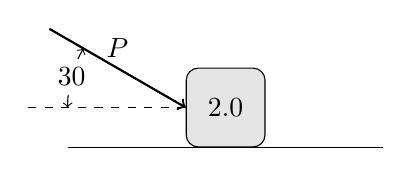
\begin{tikzpicture}
        %% Floor
        \draw (-2,0) -- (2,0);
        %% Mass
        \node[draw,fill=white!90!black,rectangle,rounded corners=1ex,minimum size=1cm,anchor=south] (A) at (0,0) {\SI{2.0}{\kilo\gram}};
        %% Forces
        \draw[dashed] (A.west) -- ++(180:2);
        \draw[<->] (A.west) ++ (180:1.5) arc (180:150:1.5) node[pos=0.5,anchor=center,fill=white] {\ang{30}};
        \draw[thick,<-] (A.west) -- ++(150:2) node[pos=0.5,anchor=south] {$P$};
    \end{tikzpicture}
    \end{center}
    A force ($P=\SI{6.0}{\newton}$) is applied to the block as shown. 
    The magnitude of the block's acceleration is \SI{1.2}{\meter\per\second\squared}.
    What is the magnitude of the force of friction acting on the block?
    \begin{multicols}{3}
    \begin{choices}
        \wrongchoice{\SI{2.0}{\newton}}
        \wrongchoice{\SI{1.4}{\newton}}
        \wrongchoice{\SI{1.6}{\newton}}
      \correctchoice{\SI{2.8}{\newton}}
        \wrongchoice{\SI{3.4}{\newton}}
    \end{choices}
    \end{multicols}
\end{question}
}

\element{serway-mc}{
\begin{question}{serway-ch05-q73}
    A \SI{3.0}{\kilo\gram} block slides on a rough horizontal surface. 
    A force of \SI{8.0}{\newton} acting parallel to the surface is applied to the block. 
    The coefficient of kinetic friction between the block and the surface is \num{0.15}. 
    What is the magnitude of the block's acceleration?
    \begin{multicols}{3}
    \begin{choices}
        \wrongchoice{\SI{1.9}{\meter\per\second\squared}}
      \correctchoice{\SI{1.2}{\meter\per\second\squared}}
        \wrongchoice{\SI{2.3}{\meter\per\second\squared}}
        \wrongchoice{\SI{1.5}{\meter\per\second\squared}}
        \wrongchoice{\SI{2.9}{\meter\per\second\squared}}
    \end{choices}
    \end{multicols}
\end{question}
}

\element{serway-mc}{
\begin{question}{serway-ch05-q74}
    A \SI{1.0}{\kilo\gram} block is pushed up a rough \ang{22} inclined plane by a force of \SI{7.0}{\newton} acting parallel to the incline. 
    The acceleration of the block is \SI{1.4}{\meter\per\second\squared} up the incline.
    Determine the magnitude of the force of friction acting on the block.
    \begin{multicols}{3}
    \begin{choices}
      \correctchoice{\SI{1.9}{\newton}}
        \wrongchoice{\SI{2.2}{\newton}}
        \wrongchoice{\SI{1.3}{\newton}}
        \wrongchoice{\SI{1.6}{\newton}}
        \wrongchoice{\SI{3.3}{\newton}}
    \end{choices}
    \end{multicols}
\end{question}
}

\element{serway-mc}{
\begin{question}{serway-ch05-q75}
    In the figure shown, the coefficient of kinetic friction between the block and the incline is \num{0.29}.
    \begin{center}
    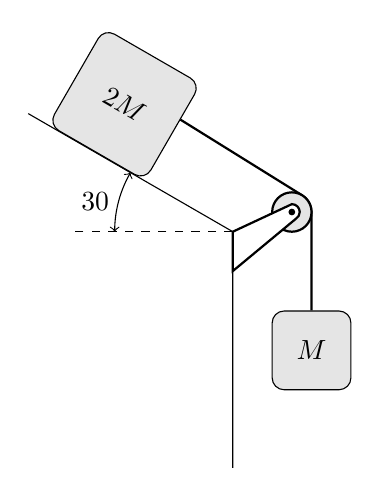
\begin{tikzpicture}
        %% Floor
        \draw (150:3) -- (0,0) -- (0,-3);
        \draw[dashed] (0,0) -- (-2,0);
        \draw[<->] (180:1.5) arc (180:150:1.5) node[pos=0.5,anchor=east] {\ang{30}};
        %% Mass
        \node[draw,fill=white!90!black,rectangle,rounded corners=1ex,minimum size=1.414cm,rotate=-30,anchor=south] (A) at (150:2) {$2M$};
        \node[draw,fill=white!90!black,rectangle,rounded corners=1ex,minimum size=1cm,anchor=north] (B) at (1,-1) {$M$};
        %% Rope and Pully
        \draw[thick] (A.south east) ++(60:0.9) -- (0.875,0.466) arc(60:0:0.25) -- (B.north);
        \draw[thick,fill=white!90!black] (0.75,0.25) circle (0.25); 
        \draw[thick,fill=white] (0,0) -- (0.75,0.35) arc (90:-60:0.1) -- (0,-0.5) -- cycle;
        \draw[fill] (0.75,0.25) circle (1pt);
    \end{tikzpicture}
    \end{center}
    What is the magnitude of the acceleration of the suspended block as it falls? 
    Disregard any pulley mass or friction in the pulley.
    \begin{multicols}{3}
    \begin{choices}
        \wrongchoice{\SI{5.4}{\meter\per\second\squared}}
        \wrongchoice{\SI{5.2}{\meter\per\second\squared}}
      \correctchoice{\SI{4.9}{\meter\per\second\squared}}
        \wrongchoice{\SI{5.6}{\meter\per\second\squared}}
        \wrongchoice{\SI{7.9}{\meter\per\second\squared}}
    \end{choices}
    \end{multicols}
\end{question}
}

\element{serway-mc}{
\begin{question}{serway-ch05-q76}
    In the figure shown, the coefficient of kinetic friction between the block and the incline is \num{0.40}.
    \begin{center}
    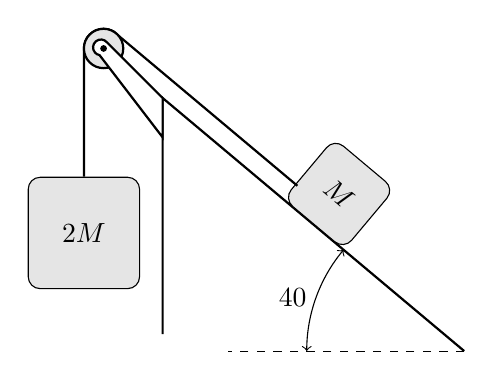
\begin{tikzpicture}
        %% Floor
        \draw[thick] (0,-3) -- (0,0) -- (320:5);
        \draw[dashed] (320:5) -- ++(180:3);
        \draw[<->] (320:5) ++(180:2) arc (180:140:2) node[pos=0.5,anchor=east] {\ang{40}};
        %% Mass
        \node[draw,fill=white!90!black,rectangle,rounded corners=1ex,minimum size=1.414cm,anchor=north] (A) at (-1,-1) {$2M$};
        \node[draw,fill=white!90!black,rectangle,rounded corners=1ex,minimum size=1cm,rotate=-40,anchor=south] (B) at (320:2.5) {$M$};
        %% Rope and Pully
        \draw[thick] (A.north) -- (-1.0,0.629) arc(180:60:0.25) -- ++(320:3.05);
        \draw[thick,fill=white!90!black] (-0.75,0.629) circle (0.25); 
        \draw[thick,fill=white] (0,0) -- ++ (135:1.0) arc (40:260:0.1) -- (0,-0.5) -- cycle;
        \draw[fill] (-0.75,0.629) circle (1pt);
    \end{tikzpicture}
    \end{center}
    What is the magnitude of the acceleration of the suspended block as it falls? 
    Disregard any pulley mass or friction in the pulley.
    \begin{multicols}{3}
    \begin{choices}
      \correctchoice{\SI{3.4}{\meter\per\second\squared}}
        \wrongchoice{\SI{3.7}{\meter\per\second\squared}}
        \wrongchoice{\SI{4.2}{\meter\per\second\squared}}
        \wrongchoice{\SI{3.9}{\meter\per\second\squared}}
        \wrongchoice{\SI{5.4}{\meter\per\second\squared}}
    \end{choices}
    \end{multicols}
\end{question}
}

\element{serway-mc}{
\begin{question}{serway-ch05-q77}
    The three blocks shown are released from rest and are observed to move with accelerations that have a magnitude of \SI{1.5}{\meter\per\second\squared}. 
    \begin{center}
    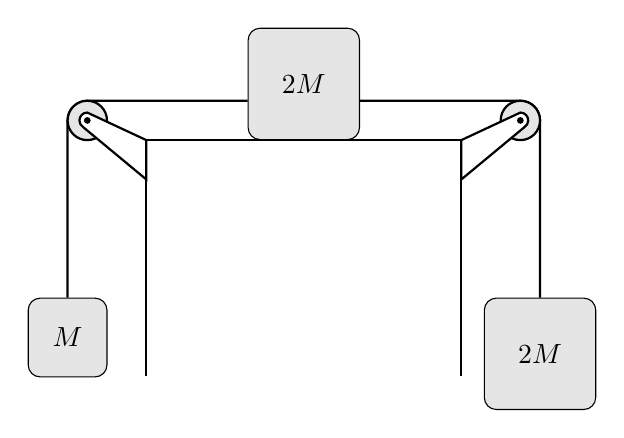
\begin{tikzpicture}
        %% Floor
        \draw[thick] (-2,-3) -- (-2,0) -- (2,0) -- (2,-3);
        %% Mass
        \node[draw,fill=white!90!black,rectangle,rounded corners=1ex,minimum size=1.414cm,anchor=south] (A) at (0,0) {$2M$};
        \node[draw,fill=white!90!black,rectangle,rounded corners=1ex,minimum size=1.414cm,anchor=north] (B) at (3,-2) {$2M$};
        \node[draw,fill=white!90!black,rectangle,rounded corners=1ex,minimum size=1.000cm,anchor=north] (C) at (-3,-2) {$M$};
        %% Rope
        \draw[thick] (A.south east) ++(90:0.5) -- (+2.75,0.5) arc(90:0:0.25) -- (B.north);
        \draw[thick] (A.south west) ++(90:0.5) -- (-2.75,0.5) arc(90:180:0.25) -- (C.north);
        %% Pully
        \draw[thick,fill=white!90!black] (+2.75,0.25) circle (0.25); 
        \draw[thick,fill=white!90!black] (-2.75,0.25) circle (0.25); 
        \draw[thick,fill=white] (2,0) -- (2.75,0.35) arc (90:-60:0.1) -- (2,-0.5) -- cycle;
        \draw[thick,fill=white] (-2,0) -- (-2.75,0.35) arc (90:240:0.1) -- (-2,-0.5) -- cycle;
        \draw[fill] (+2.75,0.25) circle (1pt);
        \draw[fill] (-2.75,0.25) circle (1pt);
    \end{tikzpicture}
    \end{center}
    What is the magnitude of the friction force on the block that slides horizontally? 
    Disregard any pulley mass or friction in the pulley and let $M=\SI{2.0}{\kilo\gram}$.
    \begin{multicols}{3}
    \begin{choices}
        \wrongchoice{\SI{6.0}{\newton}}
        \wrongchoice{\SI{5.1}{\newton}}
        \wrongchoice{\SI{5.5}{\newton}}
      \correctchoice{\SI{4.6}{\newton}}
        \wrongchoice{\SI{3.7}{\newton}}
    \end{choices}
    \end{multicols}
\end{question}
}

\element{serway-mc}{
\begin{question}{serway-ch05-q78}
    Two blocks in contact with each other are pushed to the right across a rough horizontal surface by the two forces shown. 
    \begin{center}
    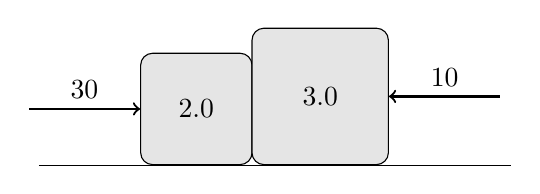
\begin{tikzpicture}
        %% Floor
        \draw (-2,0) -- (4,0);
        %% Mass
        \node[draw,fill=white!90!black,rectangle,rounded corners=1ex,minimum size=1.414cm,anchor=south] (A) at (0,0) {\SI{2.0}{\kilo\gram}};
        \node[draw,fill=white!90!black,rectangle,rounded corners=1ex,minimum size=1.732cm,anchor=south] (B) at (1.573,0) {\SI{3.0}{\kilo\gram}};
        %% Force
        \draw[thick,<-] (A.west) -- ++(180:1.414) node[pos=0.5,anchor=south] {\SI{30}{\newton}};
        \draw[thick,<-] (B.east) -- ++(0:1.414) node[pos=0.5,anchor=south] {\SI{10}{\newton}};
    \end{tikzpicture}
    \end{center}
    If the coefficient of kinetic friction between each of the blocks and the surface is \num{0.30},
        determine the magnitude of the force exerted on the \SI{2.0}{\kilo\gram} block by the \SI{3.0}{\kilo\gram} block.
    \begin{multicols}{3}
    \begin{choices}
        \wrongchoice{\SI{15}{\newton}}
        \wrongchoice{\SI{25}{\newton}}
        \wrongchoice{\SI{11}{\newton}}
      \correctchoice{\SI{22}{\newton}}
        \wrongchoice{\SI{33}{\newton}}
    \end{choices}
    \end{multicols}
\end{question}
}

\element{serway-mc}{
\begin{question}{serway-ch05-q79}
    Two blocks are accelerated across a horizontal frictionless surface as shown.
    Frictional forces keep the two blocks from sliding relative to each other,
        and the two move with the same acceleration.
    \begin{center}
    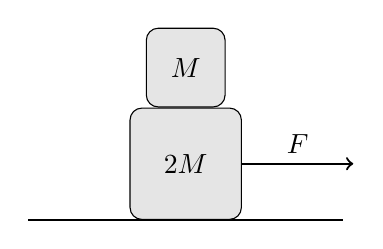
\begin{tikzpicture}
        %% Floor
        \draw (-2,0) -- (2,0);
        %% Mass
        \node[draw,fill=white!90!black,rectangle,rounded corners=1ex,minimum size=1.414cm,anchor=south] (A) at (0,0) {$2M$};
        \node[draw,fill=white!90!black,rectangle,rounded corners=1ex,minimum size=1.000cm,anchor=south] (B) at (A.north) {$M$};
        %% Force
        \draw[thick,->] (A.east) -- ++(0:1.414) node[pos=0.5,anchor=south] {$F$};
    \end{tikzpicture}
    \end{center}
    If $F=\SI{1.2}{\newton}$ and $M=\SI{1.0}{\kilo\gram}$,
        what is the horizontal component (frictional force) 
        of the force of the large block on the small block?
    \begin{multicols}{2}
    \begin{choices}
        \wrongchoice{\SI{0.40}{\newton} to the left}
        \wrongchoice{\SI{0.80}{\newton} to the right}
      \correctchoice{\SI{0.40}{\newton} to the right}
        \wrongchoice{\SI{0.80}{\newton} to the left}
        \wrongchoice{\SI{1.20}{\newton} to the left}
    \end{choices}
    \end{multicols}
\end{question}
}

\element{serway-mc}{
\begin{question}{serway-ch05-q80}
    The coefficient of kinetic friction between the surface and the larger block is \num{0.25},
        and the coefficient of kinetic friction between the surface and the smaller block is \num{0.40}.
    \begin{center}
    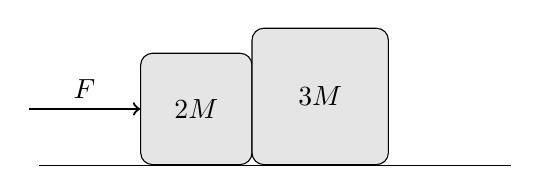
\begin{tikzpicture}
        %% Floor
        \draw (-2,0) -- (4,0);
        %% Mass
        \node[draw,fill=white!90!black,rectangle,rounded corners=1ex,minimum size=1.414cm,anchor=south] (A) at (0,0) {$2M$};
        \node[draw,fill=white!90!black,rectangle,rounded corners=1ex,minimum size=1.732cm,anchor=south] (B) at (1.573,0) {$3M$};
        %% Force
        \draw[thick,<-] (A.west) -- ++(180:1.414) node[pos=0.5,anchor=south] {$F$};
    \end{tikzpicture}
    \end{center}
    If $F=\SI{22}{\newton}$ and $M=\SI{1.0}{\kilo\gram}$ in the figure,
        what is the magnitude of the acceleration of either block?
    \begin{multicols}{3}
    \begin{choices}
        \wrongchoice{\SI{1.8}{\meter\per\second\squared}}
        \wrongchoice{\SI{2.6}{\meter\per\second\squared}}
      \correctchoice{\SI{1.4}{\meter\per\second\squared}}
        \wrongchoice{\SI{2.2}{\meter\per\second\squared}}
        \wrongchoice{\SI{3.7}{\meter\per\second\squared}}
    \end{choices}
    \end{multicols}
\end{question}
}

\element{serway-mc}{
\begin{question}{serway-ch05-q81}
    In the figure, the coefficient of kinetic friction between the surface and the larger block is \num{0.20},
        and the coefficient of kinetic friction between the surface and the smaller block is \num{0.30}. 
    \begin{center}
    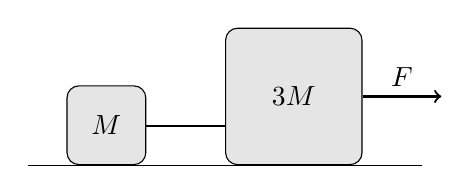
\begin{tikzpicture}
        %% Floor
        \draw (-2,0) -- (3,0);
        %% Mass
        \node[draw,fill=white!90!black,rectangle,rounded corners=1ex,minimum size=1.000cm,anchor=south east] (A) at (-0.5,0) {$M$};
        \node[draw,fill=white!90!black,rectangle,rounded corners=1ex,minimum size=1.732cm,anchor=south west] (B) at (+0.5,0) {$3M$};
        %% Force
        \draw[thick] (A.south east) ++(90:0.5) -- ++(0:1);
        \draw[thick,->] (B.east) -- ++(0:1.0) node[pos=0.5,anchor=south] {$F$};
    \end{tikzpicture}
    \end{center}
    If $F=\SI{14}{\newton}$ and $M=\SI{1.0}{\kilo\gram}$,
        what is the magnitude of the acceleration of either block?
    \begin{multicols}{3}
    \begin{choices}
        \wrongchoice{\SI{2.0}{\meter\per\second\squared}}
      \correctchoice{\SI{1.3}{\meter\per\second\squared}}
        \wrongchoice{\SI{1.5}{\meter\per\second\squared}}
        \wrongchoice{\SI{1.8}{\meter\per\second\squared}}
        \wrongchoice{\SI{3.5}{\meter\per\second\squared}}
    \end{choices}
    \end{multicols}
\end{question}
}

\element{serway-mc}{
\begin{question}{serway-ch05-q82A}
    Two blocks are accelerated across a horizontal frictionless surface as shown.
    Frictional forces keep the two blocks from sliding relative to each other,
        and the two move with the same acceleration. 
    \begin{center}
    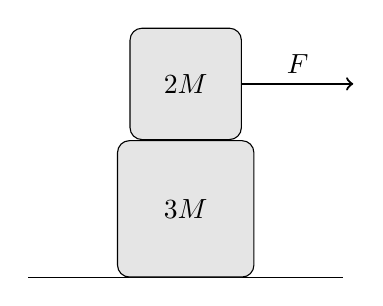
\begin{tikzpicture}
        %% Floor
        \draw (-2,0) -- (2,0);
        %% Mass
        \node[draw,fill=white!90!black,rectangle,rounded corners=1ex,minimum size=1.732cm,anchor=south] (A) at (0,0) {$3M$};
        \node[draw,fill=white!90!black,rectangle,rounded corners=1ex,minimum size=1.414cm,anchor=south] (B) at (A.north) {$2M$};
        %% Force
        \draw[thick,->] (B.east) -- ++(0:1.414) node[pos=0.5,anchor=south] {$F$};
    \end{tikzpicture}
    \end{center}
    If $F=\SI{1.2}{\newton}$ and $M=\SI{1.0}{\kilo\gram}$,
        what is the horizontal component (frictional force)
        of the force of the small block on the large block?
    \begin{multicols}{2}
    \begin{choices}
        \wrongchoice{\SI{0.48}{\newton} to the right}
      \correctchoice{\SI{0.72}{\newton} to the right}
        \wrongchoice{\SI{0.72}{\newton} to the left}
        \wrongchoice{\SI{0.48}{\newton} to the left}
        \wrongchoice{\SI{0.65}{\newton} to the left}
    \end{choices}
    \end{multicols}
\end{question}
}

\element{serway-mc}{
\begin{question}{serway-ch05-q82B}
    Two blocks are accelerated across a horizontal frictionless surface as shown.
    Frictional forces keep the two blocks from sliding relative to each other,
        and the two move with the same acceleration. 
    \begin{center}
    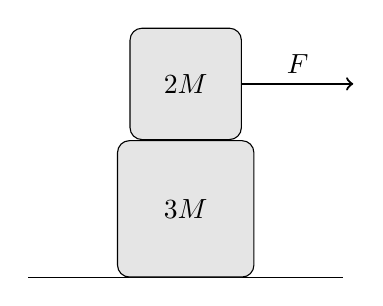
\begin{tikzpicture}
        %% Floor
        \draw (-2,0) -- (2,0);
        %% Mass
        \node[draw,fill=white!90!black,rectangle,rounded corners=1ex,minimum size=1.732cm,anchor=south] (A) at (0,0) {$3M$};
        \node[draw,fill=white!90!black,rectangle,rounded corners=1ex,minimum size=1.414cm,anchor=south] (B) at (A.north) {$2M$};
        %% Force
        \draw[thick,->] (B.east) -- ++(0:1.414) node[pos=0.5,anchor=south] {$F$};
    \end{tikzpicture}
    \end{center}
    If $F=\SI{1.2}{\newton}$ and $M=\SI{1.0}{\kilo\gram}$,
        what is the horizontal component (frictional force)
        of the force of the large block on the small block?
    \begin{multicols}{2}
    \begin{choices}
        \wrongchoice{\SI{0.48}{\newton} to the right}
        \wrongchoice{\SI{0.72}{\newton} to the right}
      \correctchoice{\SI{0.72}{\newton} to the left}
        \wrongchoice{\SI{0.48}{\newton} to the left}
        \wrongchoice{\SI{0.65}{\newton} to the left}
    \end{choices}
    \end{multicols}
\end{question}
}

\element{serway-mc}{
\begin{question}{serway-ch05-q83}
    Two blocks connected by a string are pulled across a horizontal surface by a force applied to one of the blocks,
        as shown. 
    The coefficient of kinetic friction between the blocks and the surface is \num{0.25}. 
    \begin{center}
    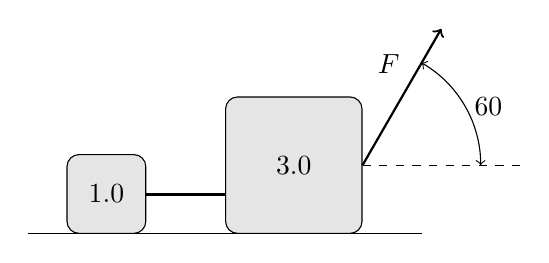
\begin{tikzpicture}
        %% Floor
        \draw (-2,0) -- (3,0);
        %% Mass
        \node[draw,fill=white!90!black,rectangle,rounded corners=1ex,minimum size=1.000cm,anchor=south east] (A) at (-0.5,0) {\SI{1.0}{\kilo\gram}};
        \node[draw,fill=white!90!black,rectangle,rounded corners=1ex,minimum size=1.732cm,anchor=south west] (B) at (+0.5,0) {\SI{3.0}{\kilo\gram}};
        \draw[thick] (A.south east) ++(90:0.5) -- ++(0:1);
        %% Force
        \draw[dashed] (B.east) -- ++(0:2);
        \draw[thick,->] (B.east) -- ++(60:2) node[pos=0.6,anchor=south east] {$F$};
        \draw[<->] (B.east) ++(0:1.5) arc (0:60:1.5) node[pos=0.5,anchor=west] {\ang{60}};
    \end{tikzpicture}
    \end{center}
    If each block has an acceleration of \SI{2.0}{\meter\per\second\squared} to the right,
        what is the magnitude $F$ of the applied force?
    \begin{multicols}{3}
    \begin{choices}
      \correctchoice{\SI{25}{\newton}}
        \wrongchoice{\SI{18}{\newton}}
        \wrongchoice{\SI{11}{\newton}}
        \wrongchoice{\SI{14}{\newton}}
        \wrongchoice{\SI{7.0}{\newton}}
    \end{choices}
    \end{multicols}
\end{question}
}

\element{serway-mc}{
\begin{question}{serway-ch05-q84}
    In the figure,
        the coefficient of kinetic friction between the surface and the larger block is \num{0.20},
        and the coefficient of kinetic friction between the surface and the smaller block is \num{0.30}. 
    \begin{center}
    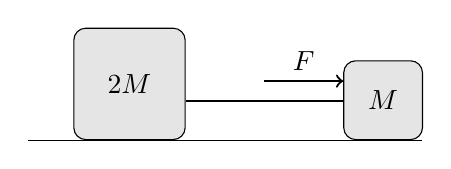
\begin{tikzpicture}
        %% Floor
        \draw (-3,0) -- (2,0);
        %% Mass
        \node[draw,fill=white!90!black,rectangle,rounded corners=1ex,minimum size=1.414cm,anchor=south east] (A) at (-1.00,0) {$2M$};
        \node[draw,fill=white!90!black,rectangle,rounded corners=1ex,minimum size=1.000cm,anchor=south west] (B) at (+1.00,0) {$M$};
        \draw[thick] (A.south east) ++(90:0.5) -- ++(0:2.0);
        %% Force
        \draw[thick,<-] (B.south west) ++ (90:0.75) -- ++(180:1) node[pos=0.5,anchor=south] {$F$};
    \end{tikzpicture}
    \end{center}
    If $F=\SI{10}{\newton}$ and $M=\SI{1.0}{\kilo\gram}$,
        what is the tension in the connecting string?
    \begin{multicols}{3}
    \begin{choices}
        \wrongchoice{\SI{8.0}{\newton}}
      \correctchoice{\SI{6.0}{\newton}}
        \wrongchoice{\SI{6.7}{\newton}}
        \wrongchoice{\SI{8.7}{\newton}}
        \wrongchoice{\SI{3.0}{\newton}}
    \end{choices}
    \end{multicols}
\end{question}
}

\element{serway-mc}{
\begin{question}{serway-ch05-q85}
    The frictional force of the floor on a large suitcase is least when the suitcase is:
    \begin{choices}
        \wrongchoice{pushed by a force parallel to the floor.}
        \wrongchoice{dragged by a force parallel to the floor.}
      \correctchoice{pulled by a force directed at an angle $\theta$ above the floor.}
        \wrongchoice{pushed by a force directed at an angle $\theta$ into the floor.}
        \wrongchoice{turned on its side and pushed by a force parallel to the floor.}
    \end{choices}
\end{question}
}

\element{serway-mc}{
\begin{question}{serway-ch05-q86}
    A \SI{60}{\kilo\gram} person rides down an icy hill of \ang{20} slope while standing on a \SI{3.0}{\kilo\gram} flat-bottomed bathroom scale. 
    Assume there is no frictional force between the bottom of the scale and the hill. 
    The static friction force the scale exerts on the person is:
    \begin{multicols}{3}
    \begin{choices}
      \correctchoice{\SI{0}{\newton}.}
        \wrongchoice{\SI{201}{\newton}.}
        \wrongchoice{\SI{211}{\newton}.}
        \wrongchoice{\SI{553}{\newton}.}
        \wrongchoice{\SI{580}{\newton}.}
    \end{choices}
    \end{multicols}
\end{question}
}

\element{serway-mc}{
\begin{question}{serway-ch05-q87}
    A chair is placed on a rug. 
    Then a book is placed on the chair. 
    The floor exerts a normal force:
    \begin{choices}
        \wrongchoice{on all three.}
        \wrongchoice{only on the book.}
        \wrongchoice{only on the rug.}
      \correctchoice{upwards on the rug and downwards on the chair.}
        \wrongchoice{only on the objects you have defined to be part of the system.}
    \end{choices}
\end{question}
}

\newcommand{\serwayChFiveQEightEight}{
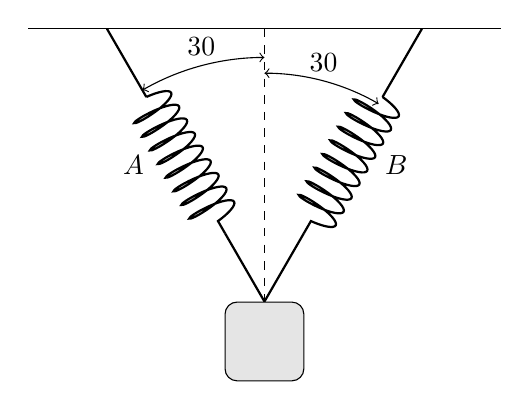
\begin{tikzpicture}
    %% Nodes
    \coordinate (A) at (-2,0);
    \coordinate (B) at (+2,0);
    \coordinate (C) at (0,-3.464);
    %% Ceiling
    \draw (-3,0) -- (3,0);
    %% Springs
    \draw[thick] (A) -- ++(300:1);
    \draw[thick,decoration={aspect=0.2,segment length=2.0mm,amplitude=3mm,coil},decorate]
        (A) ++(300:1) -- ++(300:2) node[pos=0.5,anchor=east,xshift=-4mm] {$A$};
    \draw[thick] (A) ++(300:3) --(C);
    \draw[thick] (B) -- ++(240:1);
    \draw[thick,decoration={aspect=0.2,segment length=2.0mm,amplitude=3mm,coil},decorate]
        (B) ++(240:1) -- ++(240:2) node[pos=0.5,anchor=west,xshift=4mm] {$B$};
    \draw[thick] (B) ++(240:3) --(C);
    \draw[dashed] (0,0) -- (C);
    %% Angles
    \draw[<->] (C) ++(60:2.9) arc(60:90:2.9) node[pos=0.5,anchor=south] {\ang{30}};
    \draw[<->] (C) ++(120:3.1) arc(120:90:3.1) node[pos=0.5,anchor=south] {\ang{30}};
    %\draw[<->] (C) ++ (90:2) arc (90:130:2cm) node[pos=0.5,anchor=south] {\ang{40}};
    %% Mass
    \node[draw,fill=white!90!black,rectangle,rounded corners=1ex,minimum size=1cm,anchor=north] (M) at (C) {};
\end{tikzpicture}
}

\element{serway-mc}{
\begin{question}{serway-ch05-q88}
    Two identical springs with spring constant \SI{50}{\newton\per\meter} support a \SI{5.0}{\newton} weight as in the picture below. 
    \begin{center}
        \serwayChFiveQEightEight
    \end{center}
    What is the tension in spring A?  
    \begin{multicols}{3}
    \begin{choices}
        \wrongchoice{\SI{1.45}{\newton}}
        \wrongchoice{\SI{2.50}{\newton}}
      \correctchoice{\SI{2.89}{\newton}}
        \wrongchoice{\SI{3.75}{\newton}}
        \wrongchoice{\SI{5.00}{\newton}}
    \end{choices}
    \end{multicols}
\end{question}
}

\element{serway-mc}{
\begin{question}{serway-ch05-q89}
    Two identical springs with spring constant \SI{50}{\newton\per\meter} support a \SI{5.0}{\newton} weight as in the picture below. 
    \begin{center}
        \serwayChFiveQEightEight
    \end{center}
    What is the change in length of each spring when the weight is hung on the springs.?
    \begin{multicols}{3}
    \begin{choices}
        \wrongchoice{\SI{2.9}{\centi\meter}}
        \wrongchoice{\SI{5.0}{\centi\meter}}
      \correctchoice{\SI{5.8}{\centi\meter}}
        \wrongchoice{\SI{7.5}{\centi\meter}}
        \wrongchoice{\SI{10.0}{\centi\meter}}
    \end{choices}
    \end{multicols}
\end{question}
}

\element{serway-mc}{
\begin{question}{serway-ch05-q90}
    A book is placed on a chair. 
    Then a videocassette is placed on the book. 
    The floor exerts a normal force:
    \begin{choices}
        \wrongchoice{on all three.}
        \wrongchoice{only on the book.}
      \correctchoice{only on the chair.}
        \wrongchoice{upwards on the chair and downwards on the book.}
        \wrongchoice{only on the objects that you have defined to be part of the system.}
    \end{choices}
\end{question}
}

\element{serway-mc}{
\begin{question}{serway-ch05-q91}
    Two bodies, $A$ and $B$, collide as shown in Figures (a) and (b) below.
    \begin{center}
    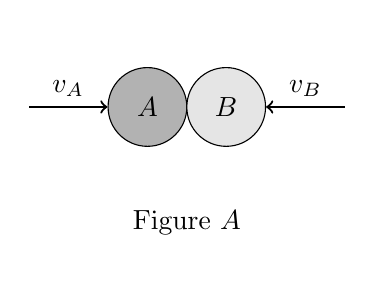
\begin{tikzpicture}
        \draw[white] (-1.75,-2) rectangle (2,1);
        \node[fill=white!70!black,draw,circle,minimum size=1cm,anchor=center] (A) at (-0.5,0) {$A$};
        \draw[thick,<-] (A.west) -- ++(180:1) node[pos=0.5,anchor=south] {$v_A$};
        \node[fill=white!90!black,draw,circle,minimum size=1cm,anchor=center] (B) at (+0.5,0) {$B$};
        \draw[thick,<-] (B.east) -- ++(0:1) node[pos=0.5,anchor=south] {$v_B$};
        \node[anchor=south] at (0,-1.75) {Figure $A$};
    \end{tikzpicture}
    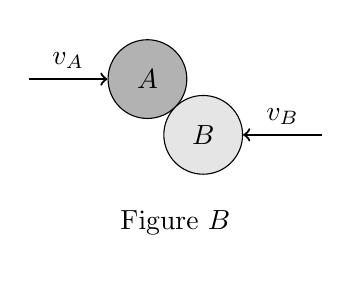
\begin{tikzpicture}
        \draw[white] (-1.75,-2) rectangle (2,1);
        \node[fill=white!70!black,draw,circle,minimum size=1cm,anchor=center] (A) at (-0.354,+0.354) {$A$};
        \draw[thick,<-] (A.west) -- ++(180:1) node[pos=0.5,anchor=south] {$v_A$};
        \node[fill=white!90!black,draw,circle,minimum size=1cm,anchor=center] (B) at (+0.354,-0.354) {$B$};
        \draw[thick,<-] (B.east) -- ++(0:1) node[pos=0.5,anchor=south] {$v_B$};
        \node[anchor=south] at (0,-1.75) {Figure $B$};
    \end{tikzpicture}
    \end{center}
    Which statement is true?
    \begin{choices}
        \wrongchoice{They exert equal and opposite forces on each other in (a) but not in (b).}
        \wrongchoice{They exert equal and opposite force on each other in (b) but not in (a).}
      \correctchoice{They exert equal and opposite force on each other in both (a) and (b).}
        \wrongchoice{The forces are equal and opposite to each other in (a), but only the components of the forces parallel to the velocities are equal in (b).}
        \wrongchoice{The forces are equal and opposite in (a), but only the components of the forces perpendicular to the velocities are equal in (b).}
    \end{choices}
\end{question}
}

\element{serway-mc}{
\begin{question}{serway-ch05-q92}
    You throw a ball up in the air and hold your hand under it to catch it when it comes down. 
    The reason why the ball stops is because:
    \begin{choices}
        \wrongchoice{your hand is there: your hand exerts no force on the ball.}
        \wrongchoice{your hand exerts a force on the ball perpendicular to its velocity.}
        \wrongchoice{your hand exerts a force on the ball in the direction of its velocity.}
      \correctchoice{your hand exerts a force on the ball in the direction opposite to its velocity.}
        \wrongchoice{your hand and the ball exert forces in the same direction on each other.}
    \end{choices}
\end{question}
}

\element{serway-mc}{
\begin{question}{serway-ch05-q93}
    You hold a tennis racket in your hand. 
    On top of the racket you have balanced a ball. 
    Which statement is true?
    \begin{choices}
        \wrongchoice{The force of your hand on the racket and the force of the ball on the racket are equal and opposite.}
        \wrongchoice{The force of the racket on your hand and the force of the ball on the racket are equal and opposite.}
        \wrongchoice{The force of your hand on the racket and the force of the racket on the ball are equal and opposite.}
        \wrongchoice{The force of the racket on your hand and the force of the racket on the ball are equal and opposite.}
      \correctchoice{The force of your hand on the racket and the force of the racket on your hand are equal and opposite.}
    \end{choices}
\end{question}
}

\element{serway-mc}{
\begin{question}{serway-ch05-q94}
    When you drag a toy teddy bear along the floor by a force that is parallel to the floor,
        the magnitude of the force of friction:
    \begin{choices}
      \correctchoice{is independent of velocity or acceleration.}
        \wrongchoice{increases when the velocity increases.}
        \wrongchoice{is proportional to the acceleration.}
        \wrongchoice{decreases when the force parallel to the floor increases.}
        \wrongchoice{increases when the force parallel to the floor increases.}
    \end{choices}
\end{question}
}

\element{serway-mc}{
\begin{question}{serway-ch05-q95}
    In order to jump off the floor,
        the floor must exert a force on you:
    \begin{choices}
        \wrongchoice{in the direction of and equal to your weight.}
        \wrongchoice{opposite to and equal to your weight.}
        \wrongchoice{in the direction of and less than your weight.}
        \wrongchoice{opposite to and less than your weight.}
      \correctchoice{opposite to and greater than your weight.}
    \end{choices}
\end{question}
}

\element{serway-mc}{
\begin{question}{serway-ch05-q96}
    When an acrobat hangs motionless from a pair of rings:
    \begin{choices}
        \wrongchoice{she has no measurable weight.}
        \wrongchoice{her weight depends on the angles the ropes make with the ceiling.}
        \wrongchoice{her weight is reduced by the upward force the rings exert on her.}
        \wrongchoice{her weight is increased by the upward force the rings exert on her.}
      \correctchoice{she exerts a gravitational force on the Earth that is equal to the sum of the forces the rings exert on her.}
    \end{choices}
\end{question}
}

\element{serway-mc}{
\begin{question}{serway-ch05-q97}
    Three boxes slide on a frictionless horizontal surface when pulled by a force of magnitude $F$. 
    \begin{center}
    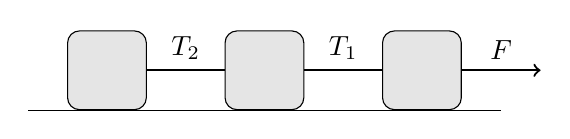
\begin{tikzpicture}
        %% Floor
        \draw (-1,0) -- (5,0);
        %% Mass
        \node[draw,fill=white!90!black,rectangle,rounded corners=1ex,minimum size=1cm,anchor=south] (A) at (0,0) {};
        \node[draw,fill=white!90!black,rectangle,rounded corners=1ex,minimum size=1cm,anchor=south] (B) at (2,0) {};
        \node[draw,fill=white!90!black,rectangle,rounded corners=1ex,minimum size=1cm,anchor=south] (C) at (4,0) {};
        %% Rope
        \draw[thick] (A.east) -- (B.west) node[pos=0.5,anchor=south] {$T_2$};
        \draw[thick] (B.east) -- (C.west) node[pos=0.5,anchor=south] {$T_1$};
        \draw[thick,->] (C.east) -- ++(0:1) node[pos=0.5,anchor=south] {$F$};
    \end{tikzpicture}
    \end{center}
    When we compare the tensions $T_1$ and $T_2$ with the force $F$, we find that:
    \begin{multicols}{2}
    \begin{choices}
        \wrongchoice{$T_1 = T_2 = F$.}
        \wrongchoice{$T_1 = F > T_2$.}
        \wrongchoice{$F > T_1 = T_2$.}
      \correctchoice{$F > T_1 > T_2$.}
        %% NOTE: parenthesis ?
        \wrongchoice{$F - T_1 < T_1 - T_2$.}
    \end{choices}
    \end{multicols}
\end{question}
}

\element{serway-mc}{
\begin{question}{serway-ch05-q98}
    Three boxes are pushed across a frictionless horizontal surface as shown. 
    \begin{center}
    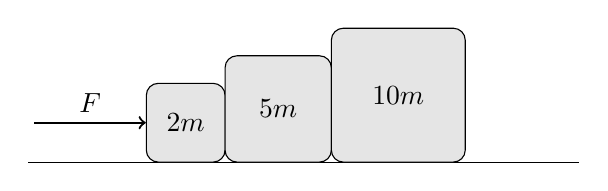
\begin{tikzpicture}
        %% Floor
        \draw (-2,0) -- (5,0);
        %% Mass
        \node[draw,fill=white!90!black,rectangle,rounded corners=1ex,minimum size=1.00cm,anchor=south] (A) at (0,0) {$2m$};
        \node[draw,fill=white!90!black,rectangle,rounded corners=1ex,minimum size=1.35cm,anchor=south] (B) at (1.175,0) {$5m$};
        \node[draw,fill=white!90!black,rectangle,rounded corners=1ex,minimum size=1.70cm,anchor=south] (C) at (2.70,0) {$10m$};
        %% Force
        \draw[thick,<-] (A.west) -- ++(180:1.414) node[pos=0.5,anchor=south] {$F$};
    \end{tikzpicture}
    \end{center}
    When we compare the normal force $N_{2,5}$ that mass $2m$ exerts on mass $5m$ with the normal force $N_{5,10}$ that mass $5m$ exerts on mass $10m$,
        we find that:
    \begin{multicols}{2}
    \begin{choices}
        \wrongchoice{$N_{2,5} = N_{5,10} = F$.}
        \wrongchoice{$N_{2,5} = F > N_{5,10}$.}
        \wrongchoice{$F > N_{2,5} = N_{5,10}$.}
      \correctchoice{$F > N_{2,5} > N_{5,10}$.}
        \wrongchoice{$F > N_{5,10} > N_{2,5}$.}
    \end{choices}
    \end{multicols}
\end{question}
}

\element{serway-mc}{
\begin{questionmult}{serway-ch05-q99}
    Given the equation 
    \begin{equation*}
        \left( \SI{2.00}{\kilo\gram} \right) \left( \SI{5.00}{\meter\per\second\squared} \right) = \SI{20.00}{\newton} - \SI{10.00}{\newton}, 
    \end{equation*}
    which answer or answers provides(s) the best description of a possible physical situation?
    \begin{choices}
      \correctchoice{A \SI{20.00}{\newton} tension pulls a \SI{2.00}{\kilo\gram} mass.  The \SI{2.00}{\kilo\gram} mass pulls another \SI{2.00}{\kilo\gram} mass.}
      \correctchoice{A \SI{20.00}{\newton} tension pushes a \SI{2.00}{\kilo\gram} mass.  The \SI{2.00}{\kilo\gram} mass pushes another \SI{2.00}{\kilo\gram} mass.}
        \wrongchoice{A \SI{2.00}{\kilo\gram} mass on a flat surface is acted on by gravity while another \SI{2.00}{\kilo\gram} mass sits on top of it.}
        %\wrongchoice{All of the situations above are possible.}
      %\correctchoice{Only (a) and (b) above are possible.}
    \end{choices}
\end{questionmult}
}

\element{serway-mc}{
\begin{question}{serway-ch05-q100}
    Given the equation 
    \begin{align*}
        \left(\SI{3.00}{\kilo\gram}\right) \left(\SI{5.88}{\meter\per\second\squared}\right) &=
        \left(\SI{3.00}{\kilo\gram}\right) \left(\SI{9.80}{\meter\per\second\squared}\right) \\
        &-\left(\SI{2.00}{\kilo\gram}\right) \left(\SI{5.88}{\meter\per\second\squared}\right) \\
    \end{align*}
    which answer or answers provides(s) the best description of a possible physical situation?
    \begin{choices}
        \wrongchoice{A \SI{3.00}{\kilo\gram} mass is suspended from the ceiling.}
        \wrongchoice{A \SI{2.00}{\kilo\gram} mass hanging over a pulley drags a \SI{3.00}{\kilo\gram} mass along a frictionless horizontal surface.}
      \correctchoice{A \SI{3.00}{\kilo\gram} mass hanging over a pulley drags a \SI{2.00}{\kilo\gram} mass along a frictionless horizontal surface.}
        \wrongchoice{A \SI{3.00}{\kilo\gram} mass hanging over a pulley drags a \SI{5.00}{\kilo\gram} mass along a frictionless horizontal surface.}
        \wrongchoice{A \SI{5.00}{\kilo\gram} mass hanging over a pulley drags a \SI{3.00}{\kilo\gram} mass along a frictionless horizontal surface.}
    \end{choices}
\end{question}
}

\element{serway-mc}{
\begin{question}{serway-ch05-q101}
    Two experiments are performed. 
    In (A), an \SI{18.0}{\newton} force pushes horizontally on a \SI{2.00}{\kilo\gram} block that then pushes on a \SI{4.00}{\kilo\gram} block. 
    In (B), an \SI{18.0}{\newton} force pushes on a \SI{4.00}{\kilo\gram} block that then pushes on a \SI{2.00}{\kilo\gram} block. 
    Which statement is correct?
    \begin{choices}
      \correctchoice{The acceleration is \SI{3.00}{\meter\per\second\squared} in both (A) and (B).}
        \wrongchoice{The acceleration is \SI{4.50}{\meter\per\second\squared} in both (A) and (B).}
        \wrongchoice{The acceleration is \SI{6.00}{\meter\per\second\squared} in both (A) and (B).}
        \wrongchoice{The acceleration is \SI{9.00}{\meter\per\second\squared} in both (A) and (B).}
        \wrongchoice{The \SI{2.00}{\kilo\gram} block has a \SI{9.00}{\meter\per\second\squared} acceleration. 
            The \SI{4.00}{\kilo\gram} block has a \SI{4.50}{\meter\per\second\squared} acceleration.}
    \end{choices}
\end{question}
}

\element{serway-mc}{
\begin{question}{serway-ch05-q102}
    A catcher arranges to catch a baseball dropped from a height \SI{50}{\meter} above his glove. 
    However, his friends substitute a soft \SI{250}{\gram} red grapefruit,
        so that it will smash apart when he catches it. 
    His glove stops the grapefruit in \SI{0.010}{\second}. 
    What force does the glove exert on the grapefruit?
    \begin{multicols}{2}
    \begin{choices}
        \wrongchoice{\SI{0.0783}{\newton}}
      \correctchoice{\SI{783}{\newton}}
        \wrongchoice{\SI{2 450}{\newton}}
        \wrongchoice{\SI{24 500}{\newton}}
        \wrongchoice{\SI{78 300}{\newton}}
    \end{choices}
    \end{multicols}
\end{question}
}

\element{serway-mc}{
\begin{question}{serway-ch05-q103}
    Jean is moving two boxes down the hall towards her dorm room. 
    The smaller box, of \SI{80}{\newton} weight, is in front of the larger box, of \SI{160}{\newton} weight. 
    She finds that she is pushing on the larger box with an \SI{84}{\newton} force. 
    Jimmy tells her that means that she is also pushing on the smaller box with an \SI{84}{\newton} force. 
    Clara tells Jimmy that he is wrong,
        because the force is divided between the two boxes in proportion to their weights as long as they have equal coefficients of kinetic friction. 
    Which one, if either, is correct, Clara or Jimmy?
    \begin{choices}
        \wrongchoice{Jimmy is correct because the larger box transmits the force to the smaller box.}
        \wrongchoice{Jimmy is correct because Jean is pushing the larger box and the 84 N force pushes the smaller box.}
      \correctchoice{Clara is correct because the applied force pushes the total mass of both boxes.}
        \wrongchoice{Clara is correct because an applied force on one of any two bodies always acts on the bodies in a 2:1 ratio.}
        \wrongchoice{Neither is correct because we cannot calculate the forces on the individual boxes.}
    \end{choices}
\end{question}
}

\newcommand{\serwayChfiveQOneZeroFour}{
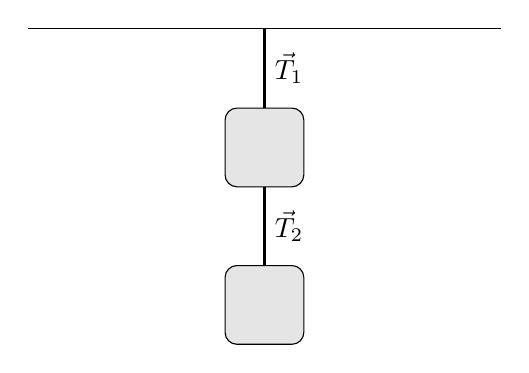
\begin{tikzpicture}
    %% Ceiling
    \draw (-3,0) -- (+3,0);
    %% Masses
    \node[draw,fill=white!90!black,rectangle,rounded corners=1ex,minimum size=1cm,anchor=north] (A) at (0,-1.0) {};
    \node[draw,fill=white!90!black,rectangle,rounded corners=1ex,minimum size=1cm,anchor=north] (B) at (0,-3.0) {};
    %% String
    \draw[thick] (0,0)  -- (A.north) node[pos=0.5,anchor=west] {$\vec{T}_1$};
    \draw[thick] (A.south)  -- (B.north) node[pos=0.5,anchor=west] {$\vec{T}_2$};
\end{tikzpicture}
}


\element{serway-mc}{
\begin{question}{serway-ch05-q104}
    A \SI{2.30}{\kilo\gram} mass is suspended from the ceiling and a \SI{1.70}{\kilo\gram} mass is suspended from the \SI{2.30}{\kilo\gram} mass, as shown. 
    \begin{center}
        \serwayChfiveQOneZeroFour
    \end{center}
    The tensions in the strings are labeled $T_1$ and $T_2$.
    A hand exerts an upward force of \SI{6.70}{\newton} on the \SI{1.70}{\kilo\gram} mass. 
    The magnitudes of the tensions are:
    %\begin{multicols}{2}
    \begin{choices}
        \wrongchoice{$T_1 = \SI{15.8}{\newton}$; $T_2 = \SI{10.0}{\newton}$.}
        \wrongchoice{$T_1 = \SI{15.8}{\newton}$; $T_2 = \SI{16.7}{\newton}$.}
        \wrongchoice{$T_1 = \SI{22.5}{\newton}$; $T_2 = \SI{10.0}{\newton}$.}
        \wrongchoice{$T_1 = \SI{22.5}{\newton}$; $T_2 = \SI{16.7}{\newton}$.}
      \correctchoice{$T_1 = \SI{32.5}{\newton}$; $T_2 = \SI{10.0}{\newton}$.}
    \end{choices}
    %\end{multicols}
\end{question}
}

\element{serway-mc}{
\begin{question}{serway-ch05-q105}
    A \SI{2.30}{\kilo\gram} mass is suspended from the ceiling and a \SI{1.70}{\kilo\gram} mass is suspended from the \SI{2.30}{\kilo\gram} mass, as shown. 
    \begin{center}
        \serwayChfiveQOneZeroFour
    \end{center}
    The tensions in the strings are labeled $T_1$ and $T_2$. 
    The string supporting the \SI{1.70}{\kilo\gram} mass is cut. 
    The magnitudes of the tension in string 1 before and after string 2 is cut are:
    %\begin{multicols}{2}
    \begin{choices}
        \wrongchoice{$T_{1,i} = \SI{22.5}{\newton}$; $T_{1,f} = \SI{5.80}{\newton}$.}
        \wrongchoice{$T_{1,i} = \SI{39.2}{\newton}$; $T_{1,f} = \SI{5.80}{\newton}$.}
        \wrongchoice{$T_{1,i} = \SI{22.5}{\newton}$; $T_{1,f} = \SI{22.5}{\newton}$.}
      \correctchoice{$T_{1,i} = \SI{39.2}{\newton}$; $T_{1,f} = \SI{22.5}{\newton}$.}
        \wrongchoice{$T_{1,i} = \SI{39.2}{\newton}$; $T_{1,f} = \SI{39.2}{\newton}$.}
    \end{choices}
    %\end{multicols}
\end{question}
}

\element{serway-mc}{
\begin{question}{serway-ch05-q106}
    A \SI{6.00}{\kilo\gram} block is placed on a \ang{30.0} incline and connected to another block on a \ang{36.87} incline. 
    \begin{center}
    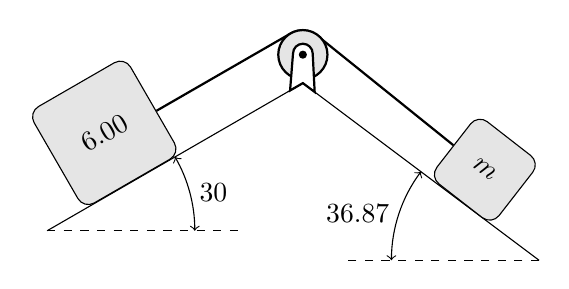
\begin{tikzpicture}[scale=1.25]
        %% Floor
        \draw (0,0) -- (323.13:3);
        \draw (0,0) -- ++(210:3);
        %% Angles
        \draw[dashed] (0,0) ++ (323.13:3) -- ++(180:2);
        \draw[<->] (0,0) ++ (323.13:3) ++(180:1.5) arc(180:143.13:1.5) node[anchor=east,pos=0.5] {\ang{36.87}};
        \draw[dashed] (0,0) ++ (210:3) -- ++(0:2);
        \draw[<->] (0,0) ++ (210:3) ++(0:1.5) arc(0:30:1.5) node[anchor=west,pos=0.5] {\ang{30}};
        %% Mass
        \node[draw,fill=white!90!black,rectangle,rounded corners=1ex,minimum size=1.414cm,anchor=south,rotate=30] (A) at (210:2) {\SI{6.00}{\kilo\gram}};
        \node[draw,fill=white!90!black,rectangle,rounded corners=1ex,minimum size=1.0cm,anchor=south,rotate=-37.87] (B) at (323.13:2) {$m$};
        %% Rope and Pully
        %% (-r sin\theta, r*tan*sin) and (0, (h-r)/cos\theta)
        \draw[thick] (A.south east) ++(120:0.50) -- (-0.125,0.504) arc(120:53.13:0.24) -- (B.west);
        \draw[thick,fill=white!90!black] (0,0.289) circle (0.25); 
        \draw[thick,fill=white] (210:0.15) -- (-0.1,0.3) arc (180:0:0.1) -- (323.13:0.15) -- (0,0) -- cycle;
        \draw[fill] (0,0.289) circle (1pt);
    \end{tikzpicture}
    \end{center}
    Although the surfaces are frictionless the blocks do not move.
    What is the mass in kilograms of the block on the \ang{36.87} incline?
    \begin{multicols}{3}
    \begin{choices}
        \wrongchoice{\SI{1.80}{\kilo\gram}}
        \wrongchoice{\SI{3.00}{\kilo\gram}}
        \wrongchoice{\SI{4.00}{\kilo\gram}}
      \correctchoice{\SI{5.00}{\kilo\gram}}
        \wrongchoice{\SI{6.00}{\kilo\gram}}
    \end{choices}
    \end{multicols}
\end{question}
}

\element{serway-mc}{
\begin{question}{serway-ch05-q107}
    A \SI{4.00}{\kilo\gram} block is suspended from the roof of an elevator. 
    A \SI{2.00}{\kilo\gram} block is suspended from the \SI{4.00}{\kilo\gram} block. 
    The tensions in strings 1 and 2 are labeled $T_1$ and $T_2$.
    \begin{center}
        \serwayChfiveQOneZeroFour
    \end{center}
    When the elevator a ccelerates upwards with an acceleration of \SI{2.20}{\meter\per\second\squared},
        the magnitudes of $T_1$ and $T_2$ are
    \begin{multicols}{2}
    \begin{choices}
        \wrongchoice{\SI{30.4}{\newton}; \SI{15.2}{\newton}.}
        \wrongchoice{\SI{39.2}{\newton}; \SI{19.6}{\newton}.}
        \wrongchoice{\SI{45.6}{\newton}; \SI{15.2}{\newton}.}
        \wrongchoice{\SI{48.0}{\newton}; \SI{24.0}{\newton}.}
      \correctchoice{\SI{72.0}{\newton}; \SI{24.0}{\newton}.}
    \end{choices}
    \end{multicols}
\end{question}
}

\element{serway-mc}{
\begin{question}{serway-ch05-q108}
    A \SI{4.00}{\kilo\gram} block is suspended from the roof of an elevator. 
    A \SI{2.00}{\kilo\gram} block is suspended from the \SI{4.00}{\kilo\gram} block. 
    The tensions in strings 1 and 2 are labeled $T_1$ and $T_2$.
    \begin{center}
        \serwayChfiveQOneZeroFour
    \end{center}
    The tensions in strings 1 and 2 are labeled $T_1$ and $T_2$.
    When the elevator accelerates downwards with an acceleration of \SI{2.20}{\meter\per\second\squared},
        the magnitudes of $T_1$ and $T_2$ are:
    \begin{multicols}{2}
    \begin{choices}
        \wrongchoice{\SI{30.4}{\newton}; \SI{15.2}{\newton}.}
      \correctchoice{\SI{39.2}{\newton}; \SI{19.6}{\newton}.}
        \wrongchoice{\SI{45.6}{\newton}; \SI{15.2}{\newton}.}
        \wrongchoice{\SI{48.0}{\newton}; \SI{24.0}{\newton}.}
        \wrongchoice{\SI{72.0}{\newton}; \SI{24.0}{\newton}.}
    \end{choices}
    \end{multicols}
\end{question}
}

\element{serway-mc}{
\begin{question}{serway-ch05-q109}
    Aline and Charlie are arguing as to whether or not it is possible in principle
        for an elevator to have an acceleration of magnitude greater than $g$. 
    In the course of their discussion they come up with the statements below. 
    Which one is correct?
    \begin{choices}
        \wrongchoice{No, because once $|\mathbf{a}|$ reaches $g$, the elevator is in free fall.}
        \wrongchoice{No, because an acceleration greater than $g$ is not possible.}
        \wrongchoice{Yes because it can reach an acceleration greater than $g$ when the cable breaks.}
      \correctchoice{Yes, because it can reach an acceleration greater than $g$ if the motor is strong enough.}
        \wrongchoice{No, because it cannot exceed its terminal acceleration.}
    \end{choices}
\end{question}
}


\endinput


